\documentclass[9pt,twocolumn,twoside]{BioRxiv}
% Use the documentclass option 'lineno' to view line numbers
\setlength{\marginparwidth}{2cm}
\usepackage[textsize=tiny,colorinlistoftodos]{todonotes} % comments in margins
\definecolor{cornflowerblue}{rgb}{0.39, 0.58, 0.93}
\usepackage{blindtext}


%%%%%%%Add comments in color
\newcommand{\citex}[1]{{\small \textcolor{red}{CITE(#1)}}}
\newcommand{\X}{{\textcolor{red}{X}}}

\newcolumntype{b}{X}
\newcolumntype{s}{>{\hsize=.5\hsize}X}

% Set supplement numbers to S and start counting newly
\newcommand{\beginsupplement}{%
        \setcounter{table}{0}
        \renewcommand{\thetable}{S\arabic{table}}%
        \setcounter{figure}{0}
        \renewcommand{\thefigure}{S\arabic{figure}}%
     }


\usepackage{hyperref}

\newcommand{\jri}[1]{\textcolor{blue}{[\begin{tiny}\textbf{JRI:} {#1}\end{tiny}]}}
\newcommand{\gmj}[1]{\textcolor{orange}{[\begin{tiny}\textbf{GMJ:} {#1}\end{tiny}]}}
\newcommand{\rra}[1]{\textcolor{red}{[\begin{tiny}\textbf{rra:} {#1}\end{tiny}]}}

\title{The Genetics of Phospholipid Metabolism In Maize Highland Adaptation}

\author[a,b,1]{Fausto Rodríguez-Zapata}
\author[a,1]{Allison C Barnes}
\author[b,1]{Karla Blöcher-Juárez}
\author[c]{Dan Gates}
\author[a]{Andi Kur}
\author[d]{Li Wang}
\author[e]{Sarah Jensen}
\author[b]{Juan M Estévez-Palmas}
\author[d]{Garrett M Janzen}
\author[f]{Taylor Crow}
\author[b]{Rocío Aguilar-Rangel}
\author[g]{Edgar Demesa-Arevalo}
\author[b]{Sergio Pérez-Limón}
\author[g]{Tara Skopelitis}
\author[g]{David Jackson}
\author[h]{Oliver Fiehn}
\author[f]{Daniel Runcie}
\author[e]{Edward S Buckler}
\author[c]{Jeffrey Ross-Ibarra}
\author[d]{Matthew Hufford}
\author[b,i]{Ruairidh JH Sawers}
\author[a, b, *]{Rubén Rellán-Álvarez}

\affil[a]{Department of Molecular and Structural Biochemistry, North Carolina State University, Raleigh, NC}
\affil[b]{National Laboratory of Genomics for Biodiversity, Irapuato, México}
\affil[c]{Department of Evolution and Ecology, Center for Population Biology and Genome Center, University of California, Davis, CA}
\affil[e]{US Department of Agriculture–Agricultural Research Service, Cornell University, Ithaca, NY}
\affil[f]{Department of Plant Sciences, University of California, Davis, CA}
\affil[d]{Department of Ecology, Evolution, and Organismal Biology, Iowa State University, Ames, USA}
\affil[g]{Cold Spring Harbor Laboratory, Cold Spring Harbor, NY, USA}
\affil[h]{West Coast Metabolomics Center, University of California, Davis, CA, USA}
\affil[i]{Department of Plant Science, The Pennsylvania State University, PA, USA}

\keywords{phospholipid metabolism; maize genetics; highland adaptation; convergent evolution}

\runningtitle{Phospholipid Pathway Selection in Highland Maize} % For use in the footer 

%% For the footnote.
%% Give the last name of the first author if only one author;
% \runningauthor{FirstAuthorLastname}
%% last names of both authors if there are two authors;
% \runningauthor{FirstAuthorLastname and SecondAuthorLastname}
%% last name of the first author followed by et al, if more than two authors.
\runningauthor{Rodríguez-Zapata, Barnes, Blöcher-Juárez \textit{et al.}}

\begin{abstract}
After domestication in low
%After domestication from lowland teosinte in the warm, humid Mexican southwest, maize colonized the highlands of México and South America. %In the highlands, maize was exposed to a whole range of environmental factors that differ from the site of domestication, including, among others, lower temperatures, soils with lower phosphorus availability and different biological pressures. 
%Here we present data supporting the hypothesis that glycerolipid metabolism remodeling was important in the process of maize adaptation to highlands. 
%We show results from common garden experiments in Mexican lowland and highland common gardens where we grew maize mapping populations and using quantitative biochemical genetics tools we identified major QTLs that explain the conversion of phosphatidylcholines (PCs) to lyso-phosphatidylcholines (LPCs) leading to a high PC/LPC ratio that is particularly conserved in Mexican highland landraces. 
%Using GBS data from 4000 maize landraces and whole genome sequences from another 30 landraces across the Americas we found that candidate genes underlying this QTL and others coding for PCs to/from LPCs conversions also show clear signs of selection to highlands. 
%I will present ongoing work to identify the causative SNPs on candidate genes that lead to this biochemical phenotype, their natural variation and ultimately the physiological mechanisms that are affected by it and their role in maize highland adaptation. 
\end{abstract}

\begin{document}

\maketitle
\thispagestyle{firststyle}
%\marginmark
\firstpagefootnote
\equalcontrib{1}
%\equalcontrib{2}

\correspondingauthoraffiliation{*}{Department of Molecular and Structural Biochemistry, North Carolina State University, 27607, Raleigh, NC. Email: rrellan@ncsu.edu}
\vspace{-33pt}% Only used for adjusting extra space in the left column of the first page

\section{Introduction}

%How do organisms adapt to high elevations
Elevation gradients are associated with changes in environmental factors that impose constraints on an organism's physiology. 
Organisms adapt to highland environments by selecting genetic variants that improve their physiological ability to live with lower oxygen availability \cite{Natarajan2016-pc, Yi2010-se, Bigham2010-is, Liu2019-eg}, higher UV-radiation \cite{Yang2017-gs} and lower temperatures \cite{Velotta2020-as, Cicconardi2020-gs}. 
%Low temperatures in particular impose a selective pressure against slow development.
%Maize domestication and expansion

After domestication from the wild relative teosinte parviglumis (\textit{Zea mays spp. parviglumis}) \cite{Matsuoka2002-bg,Piperno2009-fj} in the lowland, subtropical environment of the Balsas River (Guerrero, México) around 9,000 BP, maize (\textit{Zea mays spp. mays}) expanded throughout México and reached the highland valleys of central México around 6,500 BP \cite{Piperno2001-ea}. 
Maize also moved south to the lowlands \cite{Dickau2007-sg} and highlands \cite{Wang2017-bc} of Central America and South America \cite{Hilbert2017-eh}. 
This southward migration occurred swiftly, and there is evidence of maize highland adaptation in the Andes about the same time as Mexican highland adaptation \cite{Athens2016-ep, Grobman2012-pm}. 
These multiple events of maize adaptation are a good system to study the possible evolutionary and physiological mechanisms of convergent adaption to highland conditions \cite{Takuno2015-uj, Wang2020-mp}.
%Genetic evidence suggests that convergent adaptation was mainly driven by migration from an original mesoamerican highland population \cite{Wang2020-mp}. 

 %Photoperiod adaptation
In comparison to southward expansion, northward migration into the current United States, where Summer daylength is longer compared to Mexico, Central America, and South America, occurred at a much slower pace \cite{Da_Fonseca2015-zh, Swarts2017-ge}. 
This is likely due to maize photoperiod sensitivity that leads to maladaptation in long day conditions \cite{Hung2012-ms}. 
In fact, maize cultivation in northern latitudes was enabled by selection of allelic variants of genes in the photoperiod pathway that lead to a reduction of photoperiod sensitivity and flowering times \cite{Liang2018-af, Guo2018-on, Coles2010-db, Huang2018-ga, Yang2013-lg, Salvi2007-ku, Wang2017-bc, Hung2012-ms}.
Maize was introduced into Europe through two routes, first from the Caribbean to Spain \cite{Brandolini1968-eu, Brandenburg2017-ii}, which is likely the quickest latitudinal change maize experienced, second from Canada and the US with maize pre-adapted to northern latitudes and lower temperatures\cite{Brandenburg2017-ii}.

%Contribution of mexicana to highland maize adaptation.
In México, highland maize adaptation was aided by significant adaptive introgression from a second subspecies of teosinte, teosinte mexicana (\textit{Zea mays spp. mexicana}) that had already adapted to the highlands of México thousands of years after the split from teosinte \textit{parviglumis} \cite{Hufford2013-gs, Gonzalez-Segovia2019-jy}. 
Phenotypically, the most evident signs of \textit{mexicana} introgression into maize are the high levels of stem pigmentation and pubescence \cite{Lauter2004-eq} that are supposed to protect against high UV radiation and low temperatures. 
The ability to withstand low temperatures and efficiently photosynthesize in early stages of seedling development is a key component of maize highland adaptation \cite{Hardacre1980-tq} and recent RNA-Seq analysis of the effects of \textit{inv4m}, a major inversion in chromosome 4 introgressed from (\textit{mexicana}) support this hypothesis \cite{Crow2020-gene}.
\textit{inv4m} is also associated with shorter flowering times in highland maize \cite{Romero_Navarro2017-cn, Gates2019-xu}. 
Given the low growing degree unit accumulation in highland conditions, there has been selection for shorter flowering times in highland adapted maize \cite{Gates2019-xu}. 
%Adaptation to highland environmental factors like low temperature, high UV radiation also shows signs of canalization at the gene expression level as shown by allele specific expression in a temperate inbred x highland F1 grown in control conditions \cite{Aguilar-Rangel2017-rm}.
Other possible adaptive traits of \textit{mexicana} into highland maize may include adaptation to soils with low phosphorus \cite{AguirreLiguori2019-fl, Fustier2017-sl} that are characteristic of the acidic soils of the highland valleys of the Transmexican volcanic belt \cite{Krasilnikov2013-sm}.
Finally, there is evidence that early flowering alleles that confer an adaptive advantage in highland environments are also the result of highland mexicana introgression in highland maize \cite{Guo2018-on} and were further selected in northern latitudes.
%All taken together, the current data strongly suggests an important role of adaptive \textit{mexicana} introgression into highland maize that was then important for maize to adapt to northern latitudes in current USA, Canada and Northern Europe, where adaptation to low temperatures and early flowering would also be advantageous.    
%Today, maize has adapted to a wide diversity of environments and is grown in a wider geographical range than any other crop \cite{Hake2015-or}. 
%Maize has also adapted to a wide variety of uses, from the myriad culinary applications of local communities growing maize landraces particularly in México \cite{Bellon2018-cm} to the diverse range of products (from ethanol to high fructose syrup) that are produced with modern hybrids in modern agroindustrial operations. 
%The genetic changes that lead to maize domestication \cite{Doebley1995-su,Doebley1997-oy, Wang2005-by, Clark2006-xh,Dorweiler1993-ik} and maize adaptation to a wider latitudinal range  provide a relatively good understanding of the genetic regions and mechanisms that shaped maize domestication and latitudinal expansion.

Plant glycerolipids, which include phopsholipids, sulfolipids, galactolipids and other less polar lipids such as triacylglycerol, are involved in plant response to abiotic stresses typical of highland environments like low temperature and low phosphorus availability and flowering time.
%In this paper, we posit that phospholipid metabolism has had an important role in maize adaptation to highlands and more generally in maize adaptation to low temperature, low phosphorus availability and flowering time.   
%Our hypothesis is based on our current knowledge of how plants respond to a number of environmental conditions that are characteristic of highland environments and that affect phospholipid metabolism. 
In low temperature, two strategies plants use are to increase phospholipid concentration \cite{Degenkolbe2012-wf} and to reduce the levels of unsaturated fatty acids in glycerolipids \cite{Welti2002-uk, Lynch1987-ln} which may help maintain the fluidity of cell membranes.
%In cold adapted maize temperate lines and \textit{Tripsacum} species, genes involved in the phospholipid biosynthetic pathways show accelerated rates of protein sequence evolution, further supporting an important role of phospholipid metabolism across several species in cold adaptation \cite{Yan2019-tx}. 
In low phosphorus availability conditions plants tend to  degrade of phospholipids and increase the concentration of galactolipids and sulfolipids \cite{Lambers2012-an}, particularly in older leaves to free up phosphorus. 
Finally, certain species of phosphatidylcholine species, the most abundant phospholipid, can bind to Arabidopsis flowering locus T and accelerate flowering time through a yet unknown mechanism \cite{Nakamura2014-qf}. 
In fact, in maize, glycerolipid content has a high flowering time predictive power \cite{Riedelsheimer2013-bd}. 
%Furthemore, previous work in mesoamerican and South American highland maize populations used $F_{ST}$ statistics to identify loci that were under selection in both MesoAmerica and South America highland maize and showed little evidence of convergence between the two sub-continents but that glycerolipid pathways were some of the few pathways that were convergently selected in both highland environments  \cite{Takuno2015-uj}

In this paper we used several approaches to study the possible role of glycerolipid, and in particular phospholipid metabolism, in maize adaptation to highland conditions. 
Using measures of selection of glycerolipid pathways at the gene and metabolite level in different maize landrace panels, we showed that pathways involved in the synthesis and degradation of phospholipids have clear signs of convergent selection in several highland population across the Americas. 
We identified that \textit{ZmPLA1.2} (Phospholipase A1 2) and \textit{ZmLPCAT1} (lyso-phosphatidylcholine acyl-choline transferase 1) showed strong, repeated signals of selection in highland populations. 
\textit{ZmPLA1.2} and \textit{ZmLPCAT1} predicted enzymatic activities contribute to the synthesis and degradation of phosphatidylcholine are compelling candidates to explain the high phosphatidylcholine (PC)/lyso-phosphatidylcholine(LPC) ratios we observed in highland mesomaerican landraces. 
In fact, QTL analysis of phospholipid content in a temperate by Mexican highland biparental backcross revealed a major QTL explaining PC/LPC ratios that overlapped with \textit{ZmPLA1.2} and showed that a loss of function in the highland allele leads to high PC/LPC ratios. 
We further confirmed this loss of function using a CRISPR-CAS9 knockout in a temperate inbred background that phenocopied the highland allele PC/LPC ratios. 
Using data from thousands of genotyped landrace testcrosses grown in common garden experiments at different elevations in México, we showed a strong genotype by environment effect of the \textit{ZmPLA1.2} locus 
where the highland allele leads higher fitness in highland environments and reduced fitness at lower elevations. 
This GxE fitness effect is probably driven by highland \textit{ZmPLA1.2} allele that is associated with later flowering times in lowland environments and earlier flowering times in highland environments. 
\textit{ZmPLA1.2} CRISPR-Cas9 mutants grown in similar conditions to lowland environments confirmed this effect.
Lastly, we showed that the highland PT \textit{ZmPLA1.2} locus is the result of teosinte \textit{mexicana} introgression and that this introgression was further conserved in northern US and European Flints. 
These results suggest a potential beneficial effect of the \textit{ZmPLA1.2} highland allele in cold, high latitude environments where early flowering time would be advantageous.

In summary, the results presented in this paper help us understand at the physiological and molecular level how an important crop like maize adapts to the unique conditions of highland environments, the role of wild relatives introgression in this process, and the potential impact of this introgression in modern maize.

\section{Results}
\label{sec:results}

\subsection{Phospholipid pathways are under selection in  highland maize} 
We analyzed selection of glycerolipid related pathways both at the gene and metabolite level in highland maize using several approaches.
\subsubsection{Population Branch Excess analysis of glycerolipid pathway genes}. 
%We first selected glycerolipid related pathways using KEGG \cite{kanehisa2019}, CornCyc 8.0 from  Plant Metabolic Network \cite{Schlapfer2017-yl}, and by manually curating individual genes not assigned to a particular pathway but known to be involved in glycerolipid metabolism. See methods and the R packagage \verb|pgplipid| \cite{fausto_rodriguez_zapata_2020_4323410}.
We first quantified the extent of selection and convergent adaptation across different highland populations by calculating genome wide Population Branch Excess (PBE) statistic \cite{Pool2017-oa} at the SNP level in four highland populations across the Americas: Southwest US (SWUS), Mexican Highland (MH), Guatemalan Highlands (GH) and Andes (Figure \ref{Fig1}A). 
A genome wide PBE analysis of the same populations \cite{Wang2020-mp} found strong indications of convergent adaptation to highland environments across all four populations at the SNP, gene, and pathway level.
Population Branch Excess quantifies changes in allele frequencies in focal populations relative to two independent “outgroup” populations. 
We used \textit{Zea mays spp. parviglumis} as one of the outgroup populations for all four highland groups.  
The other outgroup was  Mexican lowlands  in the case of southwest US, Mexican highlands and Guatemalan highlands; and South American lowlands in the case of the Andes population. 
We then identified 594 genes and 30 pathways involved in glycerolipid metabolism. 
See \ref{sec:materials:methods} for full details. 
Within the 594 glycerolipid metabolism genes we identified a significant excess of genes that were target of selection in more than two populations (p < 2.87e – 5, Figure \ref{SupFig1}A).  
The most over-represented intersection of selected genes was SWUS-MH-GH ($p = 1  \times 10 ^{-15} $), perhaps indicating a set of genes selected specially in this geographical region compared to the Andean material and/or closer kinship between those populations and therefore less statistical independence.   
%We used this list to analyze if the enzymatic pathways involved in determining the glycerolipid makeup are under selection in highland maize and also the extent of possible convergent selection between  using the the Population Branch Excess (PBE) statistic   
%Each group contains three to six accessions from that particular highland environment and have been sequenced at an average 30X coverage \cite{Wang2017-bc, Wang2020-mp}. 
%A SNP was classified as a potential target of selection if it was in the top 5\%. 
%See \cite{Wang2020-mp} for further details on SNP outlier selection and PBE calculation in this populations. 
\begin{figure*}[h]
\begin{center}
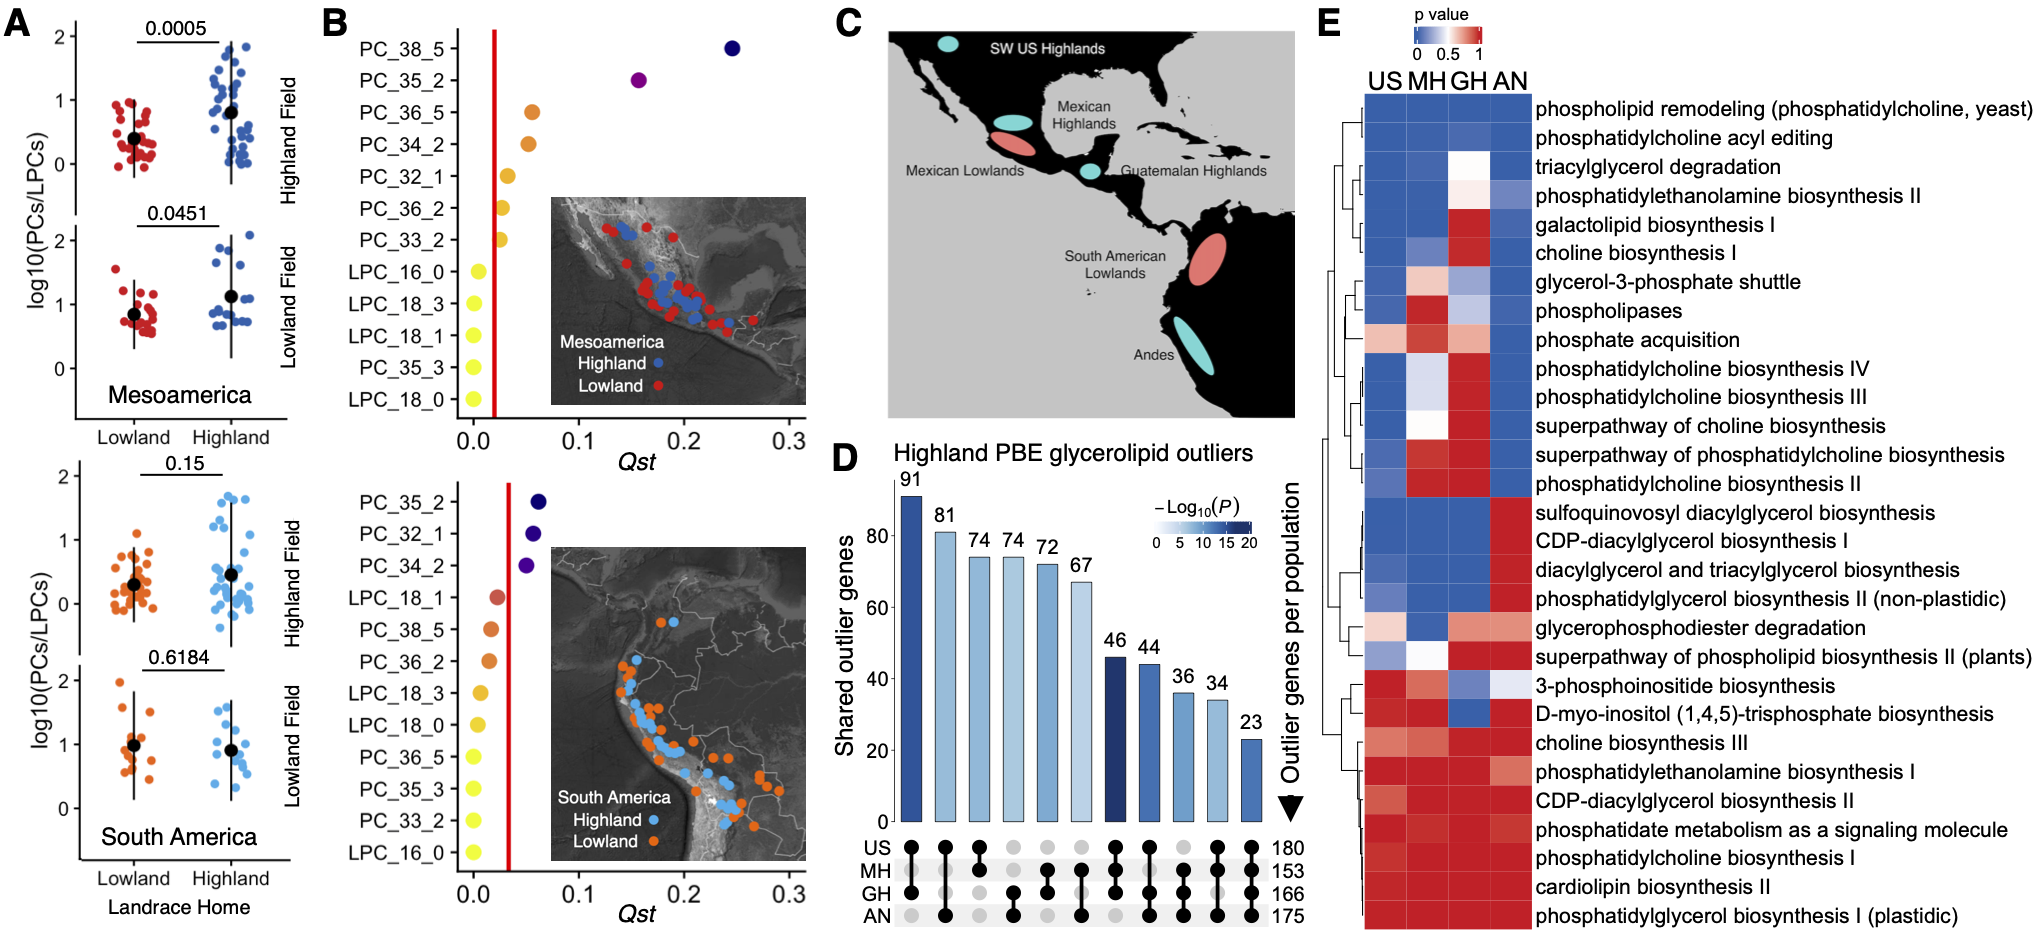
\includegraphics[width=0.7\paperwidth]{Figures/Fig_1.png}
\caption{Glycerolipid pathway selection. 
A) Populations used in the Population Branch Excess (PBE)analysis. 
B) Highland selection of Glycerolipid pathways using PBE. 
For each pathway, we first selected all SNPs in the CDS regions and 10Kb upstream and downstream of the gene and we calculated the mean pathway PBE score. 
We then constructed a null distribution by drawing 10000 samples without replacement of $n$ SNPs from those found within or around 10Kb upstream and downstream of all protein coding genes and we obtained the mean PBE for this null distribution. 
For each pathway, the heat map shows p-values corresponding to the probability of sampling from the null distribution a set of $n$ SNPs with the observed glycerolipid pathway mean PBE score or higher.
D) Map showing the geographical origin of the 120 accessions used in the common garden experiment to quantify glycerolipid levels.
E) Logarithmic values of the PCs/LPCs ratio of highland and lowland landraces from MesoAmerica and South America.
%TODO (fausto): Add Highland lowland to upper and lower "panels"
} 
\label{Fig1}
\end{center}
\end{figure*} 
%This set of phosphoglycerolipid genes is of particular interest as they might evidence convergent evolution of adaptation to highlands both in the Andes and MesoAmerica / Southwestern US.
These three populations also showed the highest number of genes that were recurrently selected in at least three populations.
We found 22 genes that are consistently PBE outliers in all four populations ($p =<1  \times  ^{-10}$). 
We then performed an independent analysis for each of the 30 pathways and compared the average pathway (10 Kb window around genes of that pathway) PBE value with a genome wide genic random sampling distribution of PBE values. 
We found that pathways involved in phosphatidylcholine (the most abundant phospholipid species in plants \cite{Gu2017-nd}, \cite{Poincelot1976-qe}, \cite{Hawke1974-ab}) remodelling (PWY-7416) and phosphatidylcholine acyl editing (PWY-6803) were significantly enriched in selection outlier genes across all four populations indicating a possible adaptive role of phospholipid remodelling in maize highland adaptation (Figure \ref{Fig1}B, Supplementary \ref{SupFig1}B and Supplementary File 1). 
Pathways involved in triacylglycerol degradation and galactolipid biosynthesis were recurrently selected in the southwest US, Mexican Highlands and the Andes while others involved in sulfolipid, diacylglycerol and phosphatidylglycerol biosynthesis were selected in the southwest US and mesoamerican populations (Figure \ref{Fig1}B).  

\textit{ZmLPCAT1} (lyso-phosphatydilcholine acyl transferase 1) is an example of a gene selected in all four populations that is part of the phospholipid remodelling and phosphatidylcholine acyl editing pathways (Supplementary File 1).
\textit{ZmLPCAT1} contains several outlier SNPs within the coding sequence of the gene that are shared across all four highland populations (Figure \ref{Fig1}C). 
%\textit{ZmLPCAT1} contains a variant previously reported to be specifically associated with flowering time in low phosphorus conditions \cite{xu2018a}. 
%In \textit{Arabidopsis}, \textit{AtLPCAT1} is a key regulator of phosphorus shoot accumulation when plants are grown under Zn deficiency conditions \cite{Kisko2018-zm}.
\textit{ZmPLA1.2} (Phospholipase A1.2) performs the reverse reaction of \textit{ZmLPCAT1} and is part of the phosphatidylcholine acyl editing, triacylglycerol degradation and phospholipases pathways. 
\textit{ZmPLA1.2} is a good example of an outlier gene in the southwest US and mesoamerican populations.
\textit{ZmPLA1.2} has particularly high PBE values in the Mexican highland population and outlier SNPs that are unique for each population and others that are shared across populations (Figure \ref{Fig1}C). 
%Variants located in the \textit{ZmPLA1.2} CDS \cite{Chen2012-gg} and 7 Kb upstream  of the gene \cite{Hung2012-ms} show significant associations with flowering time in the Nested Association Mapping population. 
%\textit{ZmPLA1.2} also showed significant associations with glycerolipid content variation in a maize lipid GWAS analysis using the European Flint and Dent inbred panels \cite{Riedelsheimer2013-bd}.

\subsubsection{Modes of convergent adaptation constraint} 
We then used Yeaman's \textit{et al.} \cite{yeaman2018} approach to evaluate the modes of convergent adaptation we observe in glycerolipid pathways across highland populations.
According to \cite{yeaman2018}, convergent adaptation may be due by a reduced number of genes that can affect a trait imposing a \textit{physiological} constraint. 
Convergent adaptation can also occur when a large number of genes may affect a trait, but pleiotropic effects limit the number of genes that effectively affect the trait imposing a a \textit{pleiotropic} constraint. 
Using Yeaman's \textit{et al.} $C_{hyper}$ statistic \cite{yeaman2018} that quantifies these two modes of convergent adaptation, we found that overall the overlap observed among the presumably adapted genes in the populations can not be explained just by physiological constraint ($C_{hyper} = 3.96$) and that most likely it includes certain degree of pleiotropic constraint, where the observed convergent adapted genes must be the least penalized by antagonistic pleiotropic effects on fitness.
The overlap was higher for the US-MesoAmerica population pairs ($C_{hyper} = 4.79$), than between the Andean and US-Mesomérica pair ($C_{hyper} = 3.14$).

\begin{table}[]
\centering
\begin{tabular}{@{}llll@{}}
\toprule
pop1 & pop2 & $C_{hyper}$   & $p$  \\ \midrule
US   & MH   & 3.82 & 1.11E-04 \\
US   & GH   & 6.17 & 8.00E-10 \\
MH   & GH   & 4.37 & 1.24E-05 \\
US   & AN   & 3.51 & 3.37E-04 \\
MH   & AN   & 2.73 & 4.43E-03 \\
GH   & AN   & 3.16 & 1.16E-03 \\ \bottomrule
\end{tabular}
\caption{Pairwise $C_{hyper}$ statistic for population comparisons.}
\label{tab:table1}
\end{table}

These results are similar to our analysis in the flowering time pathway in the same populations \cite{Wang2020-mp}. 

\subsubsection{Selection on glycerolipid metabolites} 
To evaluate if selection on genes involved in glycerophospholipid metabolism in highland maize was reflected in glycerophospholipid levels, we developed a diversity panel composed of 120 highland and lowland landraces from mesoamerica and South America (Figure \ref{Fig1}D). 
We grew this diversity panel in Mexican highland conditions in Metepec, Edo de México at 2650 masl.
We collected samples at V4-V6 and analyzed glycerolipid levels. 
Despite the intrinsic biological and environmental variability associated with analyzing open-pollinated varieties in field conditions, we could observe that highland landraces, and in particular mesoamerican highland landraces, showed  high phosphatidylcholine/lyso-phosphatidylcholine ratios, mainly due to low lyso-phosphatidylcholine levels (Figure \ref{Fig1}E). 
The differences observed in population glycerolipid levels between highland and lowland maize could the result of adaptive natural selection or random genetic drift in the process of maize adaptation to highland environments.

To distinguish between these two competing scenarios, we compared each phenotype's population variance with genetic variance of neutral markers, an approach known as a $Q_{ST}$-$F_{ST}$ comparison \cite{Leinonen2013-ic}.
$Q_{ST}$-$F_{ST}$ has been used for example to test for selection in seed metabolites between wild and domesticated wheat \cite{Beleggia2016-xw} and plant secondary metabolites in \textit{Eucalyptus} \cite{o2013chemical} and maritime pine \cite{lopez2019genetic}.
In $Q_{ST}$-$F_{ST}$ comparisons, population genetic differentiation ($F_{ST}$) is found for a set of neutral loci, and a quantitative genetic analog ($Q_{ST}$) is calculated for each phenotype of interest.
These $Q_{ST}$ values are then compared against the distribution of $F_{ST}$ values \cite{whitlock2008evolutionary}.
$Q_{ST}$ values that fall outside the distribution of $F_{ST}$ values show evidence of not being explained by neutral or random forces, but rather due to selection, either directional ($Q_{ST}$ > $F_{ST}$) or stabilizing ($Q_{ST}$ < $F_{ST}$).
%$Q_{ST}$-$F_{ST}$ comparisons can distinguish these two scenarios by comparing the within vs. between populations variance of quantitative traits ($Q_{ST}$) with that of the genetic equivalent of neutral markers ($F_{ST}$) \cite{Leinonen2013-ic}.
We calculated $Q_{ST}$-$F_{ST}$ using DartSeq genotypic data from the same plants that were used to analyze glycerolipid levels, and we calculated the $Q_{ST}$-$F_{ST}$ values for each glycerolipid species for highland/lowland populations of each subcontinent. 
Mean $Q_{ST}$ was greater than mean $F_{ST}$ in mesoamerican and South American comparisons, though two-tailed t-tests show that this difference is not statistically significant (mesoamerican comparison, p = 0.092; South American comparison, p = 0.223).
Yet, we observed several PC and LPC species with higher $Q_{ST}$ values than the neutral $F_{ST}$ in both sub continents (Supplementary Figure \ref{SupFig1}C-D, Supplementary File 2).

All together, these results further confirm that selection in genes of pathways involved in phospholipid remodelling is reflected on the glycerolipids whose levels are determined by the action of the enzymes encoded by selected genes.
\subsubsection{\textit{pcadapt} analysis of biological adaptation of Mexican landraces.} 
We then used GBS data from 2700 geo-referenced landraces from México generated by the SeeD project \cite{Romero_Navarro2017-cn, Gates2019-xu} to run a \textit{pcadapt} analysis that detects how strongly loci are contributing to patterns of differentiation between major principal components of genetic variation \cite{Luu2017-ws}.
The first principal component of \textit{pcadapt} polarized Mexican landraces based on elevation of the geographical origin of the landrace (Supplementary Figure \ref{SupFig2}A).
Using this first Principal Component we identified the outlier SNPs across the genome that are significantly associated with elevation of origin of the landrace and are potentially involved in local adaptation changes in elevation (Supplementary Figure \ref{SupFig2}B). 

\begin{figure}[h]
\begin{center}
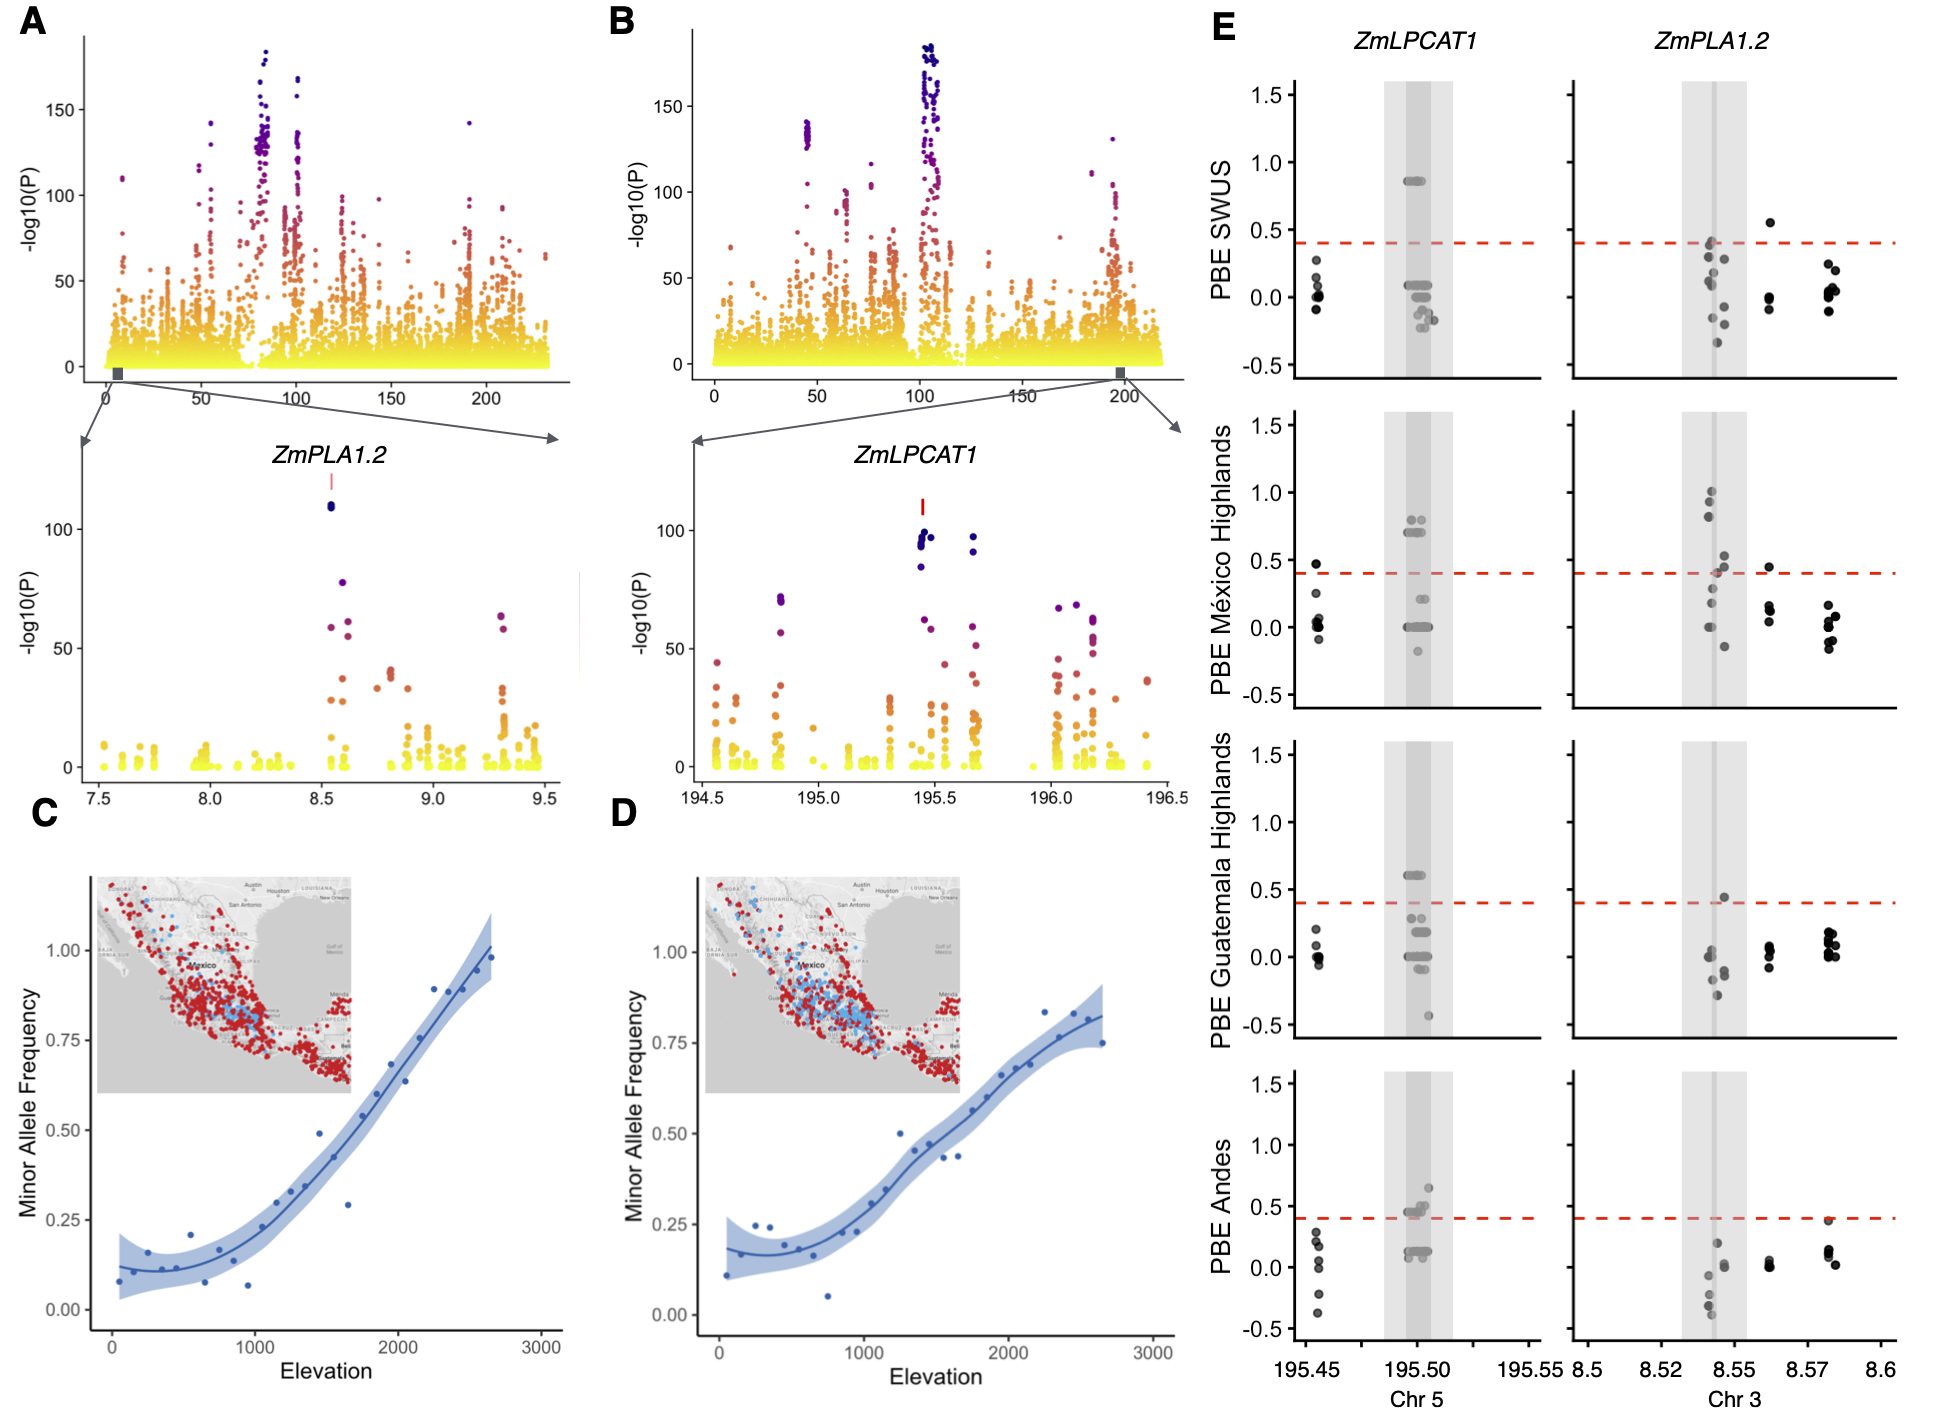
\includegraphics[width=0.4\paperwidth]{Figures/Fig_2.png}
\caption{Manhattan plots of minus log10(P‐values) \textit{Pcadapt} outliers. A) and B) \textit{Pcadapt} PC1 outliers plots of chromosome 3 and 5, respectively. 
Lower panels are zoomed areas of outlier SNPs that co-localize with the physical position of the coding sequences (marked with a red line) of \textit{ZmPLA1.2} and \textit{ZmLPCAT1}. C) and D) show the geographic and elevation dependent minor allele frequencies of the highland (blue) and lowland (red) alleles of one of the outlier SNPs in the coding sequence of \textit{ZmPLA1.2} and \textit{ZmLPCAT1}}
\label{Fig2}
\end{center}
\end{figure} 

From those genes that were PBE selection outliers in the Mexican highland population 38 were also in the top 5\% for the -log(P) values on the first \textit{pcadapt} principal component. 
This analysis also revealed that genes involved in phospholipid remodelling had significantly high -log(P) values indicating strong selection with elevation. 
Both \textit{ZmPLA1.2} and \textit{ZmLPCAT1} contained SNPs with very high \textit{pcadapt} -log10(P) values within the genes coding regions (Figure \ref{Fig2}A-B) that reflects strong elevation dependent allele frequency changes  (Figure \ref{Fig2}C-D).

All taken together, the PBE selection data, the lipodomic analysis of the 120 landrace diversity panel, the $Q_{ST}$-$F_{ST}$ analysis of lipidomics data, and the \textit{pcadapt} analysis of GBS data of thousands of geo-referenced landraces from México, strongly indicate that glycerolipid pathways and in particular those involved in phospholipid remodelling show clear signs of recurrent selection across several highland populations both at the genetic and metabolic level. 
Among these genes,\textit{ZmPLA1.2} and \textit{ZmLPCAT1}, two genes that code for enzymes performing opposite enzymatic reactions and are directly involved in the balance of PC/LPCs ratios, showed strong signals of selection in both the PBE and \textit{pcadapt} analysis.

\subsection{A major QTL explaining PC to LPC conversion overlaps with \textit{ZmPLA1.2}} 

%Our PBE and glycerolipid analysis of multiple highland and lowland populations across the Americas showed a strong signature of selection in genes involved in the synthesis and degradation of phospholipids. 
%Glycerolipid analysis of the HiLo landrace diversity panel together with $Q_{ST}$-$F_{ST}$ results further supported that high PC/LPC ratios were selected for in highland maize from MesoAmerica and to a lesser extend in South America.   
To break population structure and further characterize selection and identify loci involved in phospholipid synthesis in highland maize, we developed a Backcross Inbred  Line BC1S5 population, between B73 and Palomero Toluqueño using B73 as the recurrent parent (75\% B73, 25\% PT). 
B73 is a temperate stiff-stalk inbred line. Palomero Toluqueño (PT) accession Mexi5 (CIMMYTMA 2233) is a popcorn (Palomero means popcorn in Spanish) highland landrace from the Toluca valley in México (Figure \ref{Fig3}G) 

The B73 x PT BC1S5 mapping population was grown in triplicate on the same common garden in Metepec, Edo. de México, México as the 120 landrace diversity panel. 
The field site is located only a few kilometers away from the original collection site of the Mexi5 accession. 
In this highland conditions, with typical 5 growth degree units across the growth season, Palomero Toluqueño shows higher fitness than B73 (Figure \ref{Fig3}E-G).
While B73 typically flowers around 65 days after planting in US temperate conditions and Mexican lowland conditions B73 flowers around 150 days after planting in our Toluca field (Figure \ref{Fig3}A)
Plants were sampled at the same time as the diversity panel for glycerolipid analysis.  
Using the sum of lyso-phosphatydilcholines species (LPCs) we found a major QTL peak located at 8.5 Mb of chromosome 3 -qLPCs3- (Figure \ref{Fig3}B). 
We also found a major QTL peak -qLPCs3- when we use the sum of phosphatidylcholine species (PCs) (Figure \ref{Fig3}B). 
The PCs/LPCs ratio also showed a major QTL on the same region as qLPCs3 and qPCs3 with an even larger LOD. We searched for epistatic effects in LPCs, PCs, and PCs/LPCs rartios through a combination of \code{scantwo} and \code{stepwise} drop of found QTLs, but no additional significant peaks were found.

These QTLs were robust to environmental effects and were found in BILs grown in highland and lowland environments. 
We then seek to identify the potential candidate gene underlying the QTL. 
We hypothesized that the metabolic phenotypes we observed could probably be due to a gene with phospholipase activity. 
There are 75 genes in the maize genome with predicted phospholipase activity (Supplementary Figure\ref{SupFig4}B) and half of them have predicted PLA1 activity (Supplementary Figure\ref{SupFig4}A).  
The QTL 7.9-10 Mb 99\% confidence interval contained 72 genes. 
We identified \textit{ZmPLA1.2} (Chr3:8,542,107..8,544,078) at the QTL peak as the most likely candidate. 
\textit{ZmPLA1.2} has a predicted Phospholipase A1-Igamma1 predicted activity and can be classified, based on homology with Arabidopsis, as a PC hydrolizing PLA1 Class 1 Phospholipase \cite{Ryu2004-iv}. 
PLA1 phospholipases hydrolize phospholipids in the sn-1 position and produce a lyso-phospholipid and a fatty acid as a result (Supplementary Figure\ref{SupFig4}B). 

\begin{figure*}[h]
\begin{center}
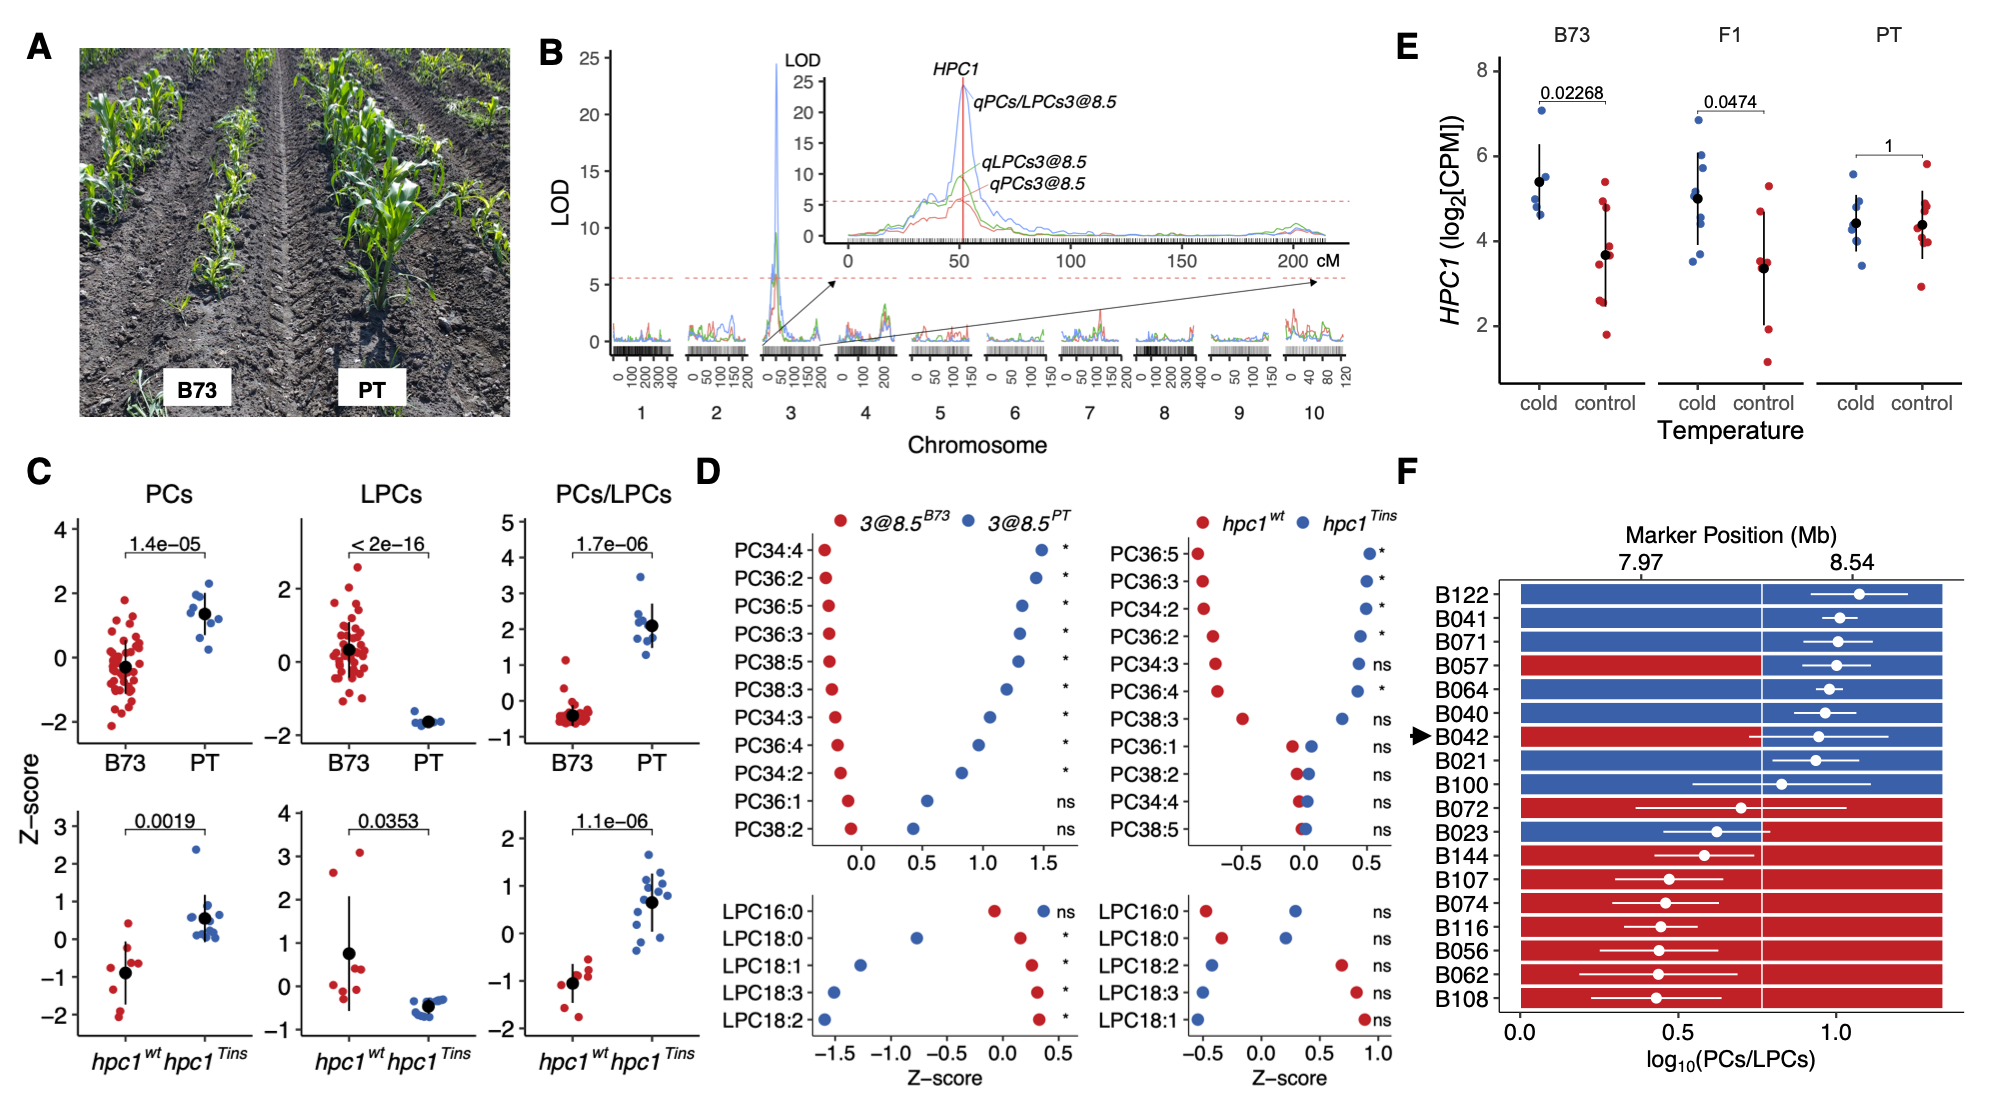
\includegraphics[width=0.8\paperwidth]{Figures/Fig_3.png}
\caption{QTL analysis of phospholipid content in a B73 x PT BIL population. 
A) PT and B73 plants growing in the highland Metepec field. 
B) QTL analysis using data collected from plants growing in the highland and lowland fields of PCs, LPCs and PCs/LPCs ratio identified overlapping major QTLs at 8.5 Mb in chromosome 3. 
QTL peak coincides with the physical location of \textit{ZmPLA1.2}. 
C)PCs, LPCs and PC/LPCs z-scores effect sizes of BILs at chr 3 8.5 Mb that are either homozygous B73 or PT (top row) and CRISPR-CAS9 \textit{ZmPLA1.2} mutant and wild plants (bottom row).        
D)Individual PCs and LPCs species z-scores effect sizes of BILs at at chr 3 8.5 Mb (top row) and CRISPR-CAS9 \textit{ZmPLA1.2} mutant}
\label{Fig3}
\end{center}
\end{figure*} 
Class 1 PLA1s phospholipases are targeted to the chloroplast. We, in fact, identified a chloroplast transit peptide at the beginning of \textit{ZmPLA1.2} and we further confirmed chloroplast localization by expressing the \textit{ZmPLA1.2} transit peptide tagged with GFP in tobacco cells (Figure\ref{Fig4}A-B, Supplementary \ref{SupFig4}C). 
In, B73, \textit{ZmPLA1.2} is one of the most highly expressed phospholipases and is highly expressed in vegetative leaves (V4-V9) (Supplementary Figure\ref{SupFig4}D) \cite{Stelpflug2016-vr}. 
\textit{ZmPLA1.2} is highly expressed in B73 and other temperate inbreds under low temperature conditions and is downregulated in heat conditions (Supplementary Figure\ref{SupFig4}E) \cite{Waters2017-nat}.
PCs, LPCs and PCs/LPCs effect sizes at genetic markers in the QTL peak (chr3 @8.54 Mb, Figure \ref{Fig3}C-D, top panels) show that homozygous PT BILs have higher PCs, lower LPCs and therefore higher PCs/LPCs ratios than homozygous B73 BILs. 
If, \textit{ZmPLA1.2} is the underlying causal gene of the QTL the metabolic phenotypes observed would be consistent with a loss or impaired function of the \textit{ZmPLA1.2-PT} allele that leads to higher levels of PCs and and low levels of LPCs in PT. 
This allele and the corresponding high PC/LPC ratio is conserved in other mesoamerican highland landraces (Figure\ref{Fig1} and \ref{Fig2}). 
We found that most of the individual LPCs at the qLPCs3 locus correspond to LPCs that at contain at least one double bond in the fatty acid (Figure  \ref{Fig3}D, Supplementary Fig \ref{Fig3}).
We then generated a CRISPR-CAS9 \textit{ZmPLA1.2} knockout mutant in B104, a temperate inbred derived from B73, and measured PC and LPC species in WT and mutant plants grown under greenhouse control conditions. 
The mutant CRISPR-CAS9 phenocopied the PT allele effect of the BILs further confirming that the \textit{ZmPLA1.2-PT} is a loss of function allele that underlies the QTL in chr3 @8.5 Mb. 
%Our PBE and \textit{pcadapt} identified \textit{ZmPLA1.2} as gene under strong selection in highland maize. 
%Our results in the landrace diversity panel also  indicated that the PCs/LPCs levels were particularly high Mexican highland landraces. 
%We further studied PC, LPC selection using the individual species and individual PC/LPC species ratio. 
%The ratio of PC to LPC is higher in BILs that are homozygous PT at the \textit{ZmPLA1.2} locus. 
%The differences are most stark in ratios where the LPC lipid species is presumably a product of the reaction, as the reaction is not occurring in PT lines. 
%For example, \textit{ZmPLA1.2} would remove a 16:0 fatty acid from PC34:1 and leave LPC18:1 behind. 

\subsection{Mode of action of \textit{ZmPLA1.2}} 
All taken together our PBE, \textit{pcaadapt}, $Q_{ST}$-$F_{ST}$ and QTL data strongly suggest the PC-LPC balance was under selection and that \textit{ZmPLA1.2} and to a minor extent\textit{ZmLPCAT1}are themselves under selection in highland maize and are major drivers of the lipid changes observed in highland maize. 
Furthermore, the QTL data suggest that the highland PT allele is a loss of function of \textit{ZmPLA1.2}. 
This loss of function could be due to a mis-regulation of the expression level in highland landraces or to a mutation affecting the enzymatic activity of ZmPLA1.2. 
We analyzed \textit{ZmPLA1.2} expression in B73, PT and the corresponding F1 in plants grown under high and low temperature simulating highland and lowland conditions (Figure \ref{Fig4}C). 
Under cold conditions \textit{ZmPLA1.2-B73} was up-regulated but \textit{ZmPLA1.2-PT} was not (Figure \ref{Fig4}C). 
F1 plants showed a similar behaviour \textit{ZmPLA1.2-B73} plants.
\textit{ZmPLA1.2} on the F1 showed a pattern of expression consistent with a dominant B73 effect and this was also the case when we analyzed PC/LPCs ratios in the few B73 x PT BC1S5 BILs that are heterozygous at the qPC/LPC@8.5 locus (Supplementary Figure \ref{SupFig5}A).
\begin{figure*}[ht]
\begin{center}
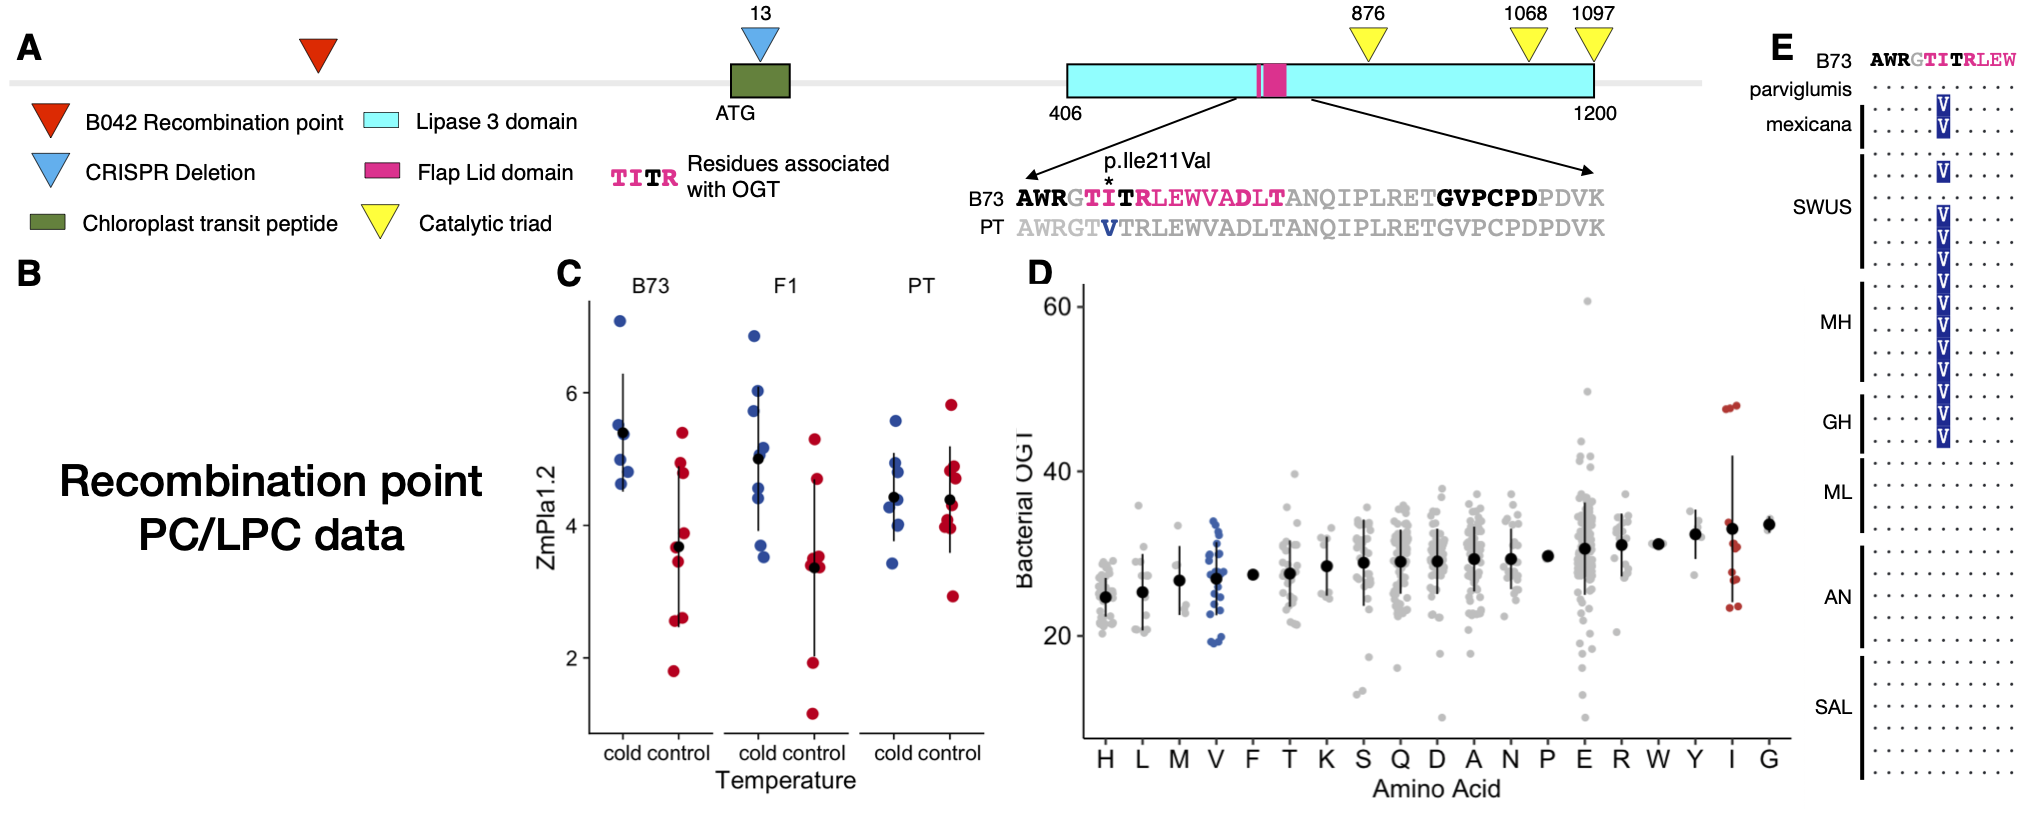
\includegraphics[width=0.8\paperwidth]{Figures/Fig_4.png}
\caption{Analysis of the underlying causes of \textit{ZmPLA1.2} variation on PC/LPC ratios.    
A) \textit{ZmPLA1.2} promoter and coding sequence showing different features. CTP represents the chloroplast transit peptide. The domains of \textit{ZmPLA1.2} were analyzed from UniProt identifier \hyperlink{https://www.uniprot.org/uniprot/A0A1D6MIA3}{A0A1D6MIA3}. The \hyperlink{https://www.ebi.ac.uk/interpro/entry/pfam/PF01764/}{PFAM domain}, and \hyperlink{https://www.ebi.ac.uk/interpro/entry/InterPro/IPR029058/}{alpha/beta Hydrolase fold} were identified using InterPro, and \hyperlink{https://www.ncbi.nlm.nih.gov/Structure/cdd/cddsrv.cgi?uid=cd00519}{Lipase3 domain}, shown in cyan, including flap lid, shown in magenta, and S293, D357, and H400 catalytic triad were identified from CDD. H416 was identified as a substitute for H400 in the catalytic triad by protein modelling.
B) Subcellular localization of \textit{ZmPLA1.2}.
C) \textit{ZmPLA1.2} Expression analysis of B73, PT and their F1 grown in control and cold temperatures in growth chamber conditions. 
D) PC/LPC ratios of several BILs including B042 that shows a recombination of event 500 bp upstream of the ATG.
E) Bacterial optimal growth temperature (OGT) of different residues at the position in the flap-lid domain where the B73/PT mutation leading to a Ile211Val conversion was identified. Across the whole lipase domain, residues in bold in the flap lid domain (A) showed high correlation with bacterial OGT. 
F) Alignments around the Ile211Val mutation in the flap-lid domain in B73, mexicana and parviglumis and highland and lowland landraces southwest US, mesoamerican highlands and lowlands and Andes and South America lowlands.} 
 
\label{Fig4}
\end{center}
\end{figure*} 
Loss of function could also be the result of enzymatic malfunction of the \textit{ZmPLA1.2-PT} allele and in fact PBE and pcadapt outliers SNPs are located within the CDS of \textit{ZmPLA1.2} and not within the regulatory region. 
To further explore nature of the metabolic effect we observed, we Sanger sequenced B73 x PT BILs (B021, B042, B122 that are homozygous PT on the \textit{ZmPLA1.2}.
We identified a recombination point 500 bases pairs upstream of the ATG of \textit{ZmPLA1.2} (Figure \ref{Fig4}A, Supplemmentary Figure \ref{SupFig6}).
BIL B104 then contains a \textit{ZmPLA1.2-PT} coding sequence and mostly \textit{ZmPLA1.2-B73} (500 base pairs upstream of the ATG) regulatory region. 
PC/LPC levels on B104 where similar to other BILs that are homozygous PT at the 8.54 Mb marker in the QTL peak (Figure \ref{Fig4}D). 
This result supports the hypothesis that the metabolic effect we see is due to a loss of function in ZmPLA1.2-PT. 
We also identified several non-synonymous SNPs within the CDS (407, 520, 553, 610, 631, 1028, 1315, 1342, and 1345 from the ATG) that could have an effect on \textit{ZmPLA1.2}.
We focused our attention on SNP 631 on the flap lid domain that leads to a conservative substitution from isoleucine to valine (Ile211Leu,Figure \ref{Fig4}A).  
The flap lid domain is located in a conserved lipase 3 domain (PFAM domain PF01764) that is highly conserved across the tree of life. 
We identified 982 observations of the PF01764 PFAM domain in 719 prokaryote species using PfamScan \cite{Potter2018-tk, El-Gebali2019-pw}.
We analyzed nucleotide diversity in the promoter and CDS of \textit{ZmPLA1.2} of highland and lowland landraces from México and South America and we did not observe any obvious pattern  when we compared highland vs lowland (Supplementary \ref{SupFig5}B). 
We then used a recent tool that uses tRNA sequences to calculate bacterial optimal growth temperatures \cite{Cimen2020-dm}.
We observed significant associations of residues that were mainly located in the flap lid region with variation in optimal growth temperatures (Figure \ref{Fig4}A), including residue 211. 
We then specifically analyzed variation in this residue and observed that the PT allele (V) was associated with lower bacterial optimal growth temperature than the B73 allele (I) (Figure \ref{Fig4}E) suggesting that the SNP we identified in PT leading to Ile211Leu may be associated with adaptation to lower temperatures that highland maize is usually exposed to. 
We then explored if this SNP was unique to PT or was conserved in other highland maize.
This SNP was not captured in the GBS dataset from Seeds so we used WGS sequenced data that we had used for PBE analysis. 
The PT allele was conserved in highland landraces from Mexico and Guatemala and was segregating in SWUS landraces. The B73 was fixed in lowland Mexican and South American and Andean landraces (Figure \ref{Fig4}F). 
These results are consistent with the PBE results we have observed before (Figure \ref{Fig1}C).
This is a typical pattern of teosinte \textit{mexicana} introgression \cite{Wang2020-mp} and indeed the PT allele was present in both teosinte \textit{mexicana} accessions sequenced in the maize Hapmap. 
The PT allele was present in 1/4 of the teosinte \textit{parviglumis} accessions on Hapmap 3 \cite{Bukowski2017-ng}. 
This lead us to ask whether the PT allele was the result of teosinte \textit{mexicana} introgression in highland maize or selected from \textit{parviglumis} standing variation in teosinte. 
\subsection{Introgression of \textit{mexicana}} 
To test for \textit{mexicana} introgression, we used \(f_d\) data from \cite{Gonzalez-Segovia2019-jy} calculated using WGS of: two PT outbred individuals, a Mushito (another highland landrace) outbred individual, two lowland landrace inbreds, Reventador and NalTel, two \textit{mexicana} inbreds, three \textit{parviglumis} inbreds and a tripsacum individual used as an outgroup. 
\(f_d\) data around the \textit{ZmPLA1.2} indicated that the region was introgressed from \textit{mexicana} into highland maize. (Figure\ref{Fig5}A).
We then performed a haplotype network analysis using SNP data of the \textit{ZmPLA1.2} CDS from X Mexican homozygous accessions from the Seed Dataset \cite{Romero_Navarro2017-cn}. 
We identified 9 haplotype groups that clustered mainly based on elevation. (Figure\ref{Fig5}B) 
The two major groups (II) and (VI) contained mainly lowland and highland landraces respectively. 
The two \textit{mexicana} liners were located in group IV together with a group of 7 highland landraces from X. (Figure\ref{Fig5}A)
%TODO(Fausto) Add details. 
We then asked if the \textit{mexicana} introgression present in mesoamerican highland maize is present in modern maize inbreds. 
To address this question we constructed phylogenetic tree using using sample of the hapmap inbred lines including lines from the 282 inbred panel and PT. 

\begin{figure*}[ht]
\begin{center}
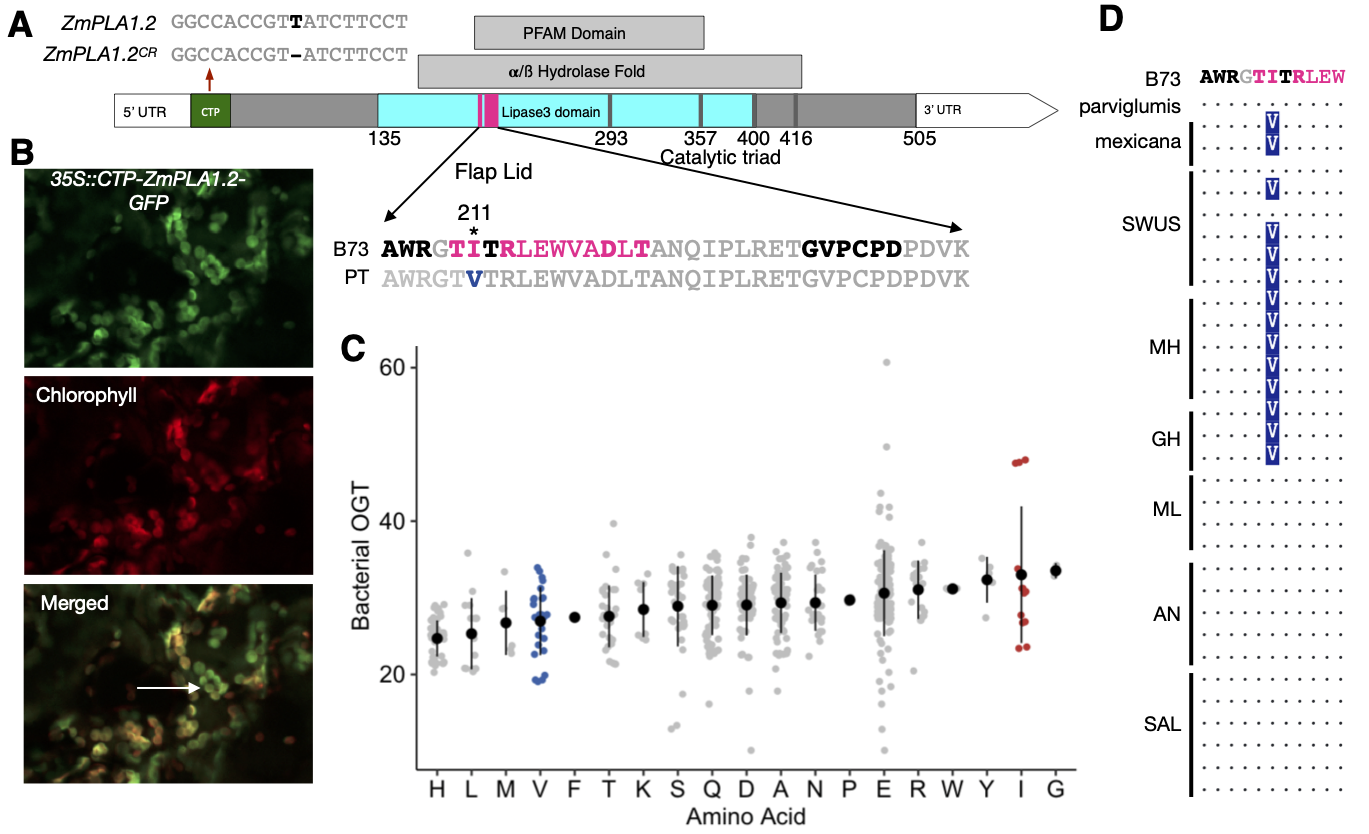
\includegraphics[width=0.8\paperwidth]{Figures/Fig_5.png}
\caption{Introgression of teosinte \textit{mexicana} into maize \textit{ZmPLA1.2}  
A) \(f_d\) analysis of \textit{mexicana} introgression. Data was obtained from \cite{Gonzalez-Segovia2019-jy}. 
B) Haplotype network analysis of \textit{ZmPLA1.2} CDS SNPs using X Mexican homozyogous individuals from the Seeds dataset.
C) Phyologenetic tree of \textit{ZmPLA1.2} CDS using a sample of hapmap inbreds and Palomero Toluqueño
D) \textit{ZmPLA1.2-PT} expression correlation with DTA in short and long days. Inbred lines from the PT lineage shown in panel C are colored in blue while inbred lines from the B73 lineage are colored in red.
Data from \cite{Kremling2018-gn}}
\label{Fig5}
\end{center}
\end{figure*} 

Palomero Toluqueño and the teosinte \textit{mexicanas} TIL-08 and TIL-25 clustered together with Northern European (Figure \ref{Fig5}C) Flints like EP1 UH008 and UH009. 
Other northern US flints like CM7 are also closely related to the \textit{mexicana} introgression. 
This data suggests that after introgression into highland maize, the \textit{ZxPla1.2} allele was conserved in Flint materials adapted to cold environments in the North of the US and Canada and Europe. 

\subsection{Fitness effects of \textit{ZmPLA1.2-PT}}

%Our results have shown that pathways and genes involved in the synthesis and degradation of phospholipids have been repeated targets of selection in several highland maize populations \ref{Fig1} and \ref{Fig2}. 
%Using PBE and \textit{pcadapt} analysis we identified \textit{ZmPLA1.2}, a gene with a predicted Phospholipase A1 activity and \textit{ZmLPCAT1} a gene with predicted lyso-phospholipid acyl-transferese activity were identified as clear highland selection outliers. 
%Furthermore, we identified clear patterns of high PC/LPC levels in highland maize landraces and high \textit{Qst-Fst} values in indvidual PC species that confirm that selection signatures at the gene level are reflected in the metabolic output of the genes under selection. 
%We then further found that in a B73 x PT Backcross mapping population the levels of PC and LPC species are controlled by a major QTL located at the physical location of \textit{ZmPLA1.2} and that he highland allele led to high PC/LPC levels consisten with loss of function or misregulation of \textit{ZmPLA1.2}. \ref{Fig3}  Introgression and phylogenetic analysis indicated \textit{ZmPLA1.2-PT} was the result of teosinte \textit{mexicana} introgression in highland maize and that this introgression is conserved in Northern European Flint inbreds.
We then explored the possible effect of genetic variation in \textit{ZmPLA1.2-PT} alleles on several fitness traits to explore the relevance of genetic variation at \textit{ZmPLA1.2-PT} maize local adaptation to highland conditions. 
\subsubsection{\textit{ZmPLA1.2}expression in modern maize is associated with flowering time}
Building on previous reports that indicate a role of PC species in determining flowering time \cite{Nakamura2014-qf, Riedelsheimer2013-bd} and considering the significant accumulation of PC species as a result of \textit{ZmPLA1.2} genetic variation we asked if \textit{ZmPLA1.2} could be associated with flowering time traits in modern maize. 
We used a large gene expression dataset obtained from the 282 maize diversity panel sampled at several developmental stages \cite{Kremling2018-gn} phenotypic datasets collected from the same panel grown in long and short day conditions. 
We found that \textit{ZmPLA1.2} and \textit{ZmLPCAT1} expression are usually inversely correlated in most of the tissues \ref{SupFig7}. further supporting the idea that these two enzymes are coregulated. 
We also found significant associations of \textit{ZmPLA1.2} with several flowering time traits in aerial tissues similar in magnitude with other well known genes that are involved in determining flowering time \ref{SupFig7} like \textit{ZmZcn8} and \textit{ZmRap2.7}.
Furthermore, in both long and short days conditions, the inbred lines that carry \textit{ZmPLA1.2-PT} allele showed lower levels of expression and shorter flowering times than the inbreds that carry the \textit{ZmPLA1.2-PT} allele  (Figure \ref{Fig5}D). 

\subsubsection{\textit{ZmPLA1.2} shows strong elevation-dependent antagonistic pleiotropy in Mexican landraces}
We then re-analyzed phenotypic data from the F1 Association Mapping (FOAM) panel of \textit{et al} \cite{Romero_Navarro2017-cn} and \cite{Gates2019-xu} and fit model to estimate the effect of \textit{ZmPLA1.2} genotype on several fitness trait's intercept and slope on trial elevation using \textit{GridLMM} \cite{Runcie2019-Gr}. We found that that genetic variation in \textit{ZmPLA1.2} showed significant effects of genotype by environment interactions on several fitness related traits. \ref{Fig6}B. 
\textit{ZmPLA1.2} showed clear antagonist pleiotropy effects on flowering time traits \ref{Fig6}A. 
The highland \textit{ZmPLA1.2-PT} allele was associated to an increase of days to anthesis (DTA) of almost one day and of ASI (Anthesis to Silking Interval) of around 1/4 of a day in low elevation environments while, at high elevations, the highland allele was associated with a decrease of DTA and ASI of 1 and 1/4 of a day, respectively.
Yield related traits suchs as field weight (combined weight of kernels and cob for an entire row measured in the field) and grain weight per hectare showed typical conditional neutrality effects where the highland allele had no effects in lowland environments but led to higher yield values in highland environments.
\subsubsection{\textit{ZmPLA1.2} CRISPR-CAS9 mutants phenocopied the effect of the highland allele in flowering time}
We then grew the \textit{ZmPLA1.2} CRISPR-CAS9 in long day conditions in North Carolina and measured flowering time. 
%Mutant plants flowered around 20 hours earlier than wild type plants. 
The mutant phenocopied the effect of the highland allele in Mexican lowland conditions where the highland allele leads to an increase of flowering time of around 1 days. 
We are currently performing further experiments in conditions simulating highland environments to test if the mutant shows a similar reduction in flowering time in the mutant confirming an interaction between \textit{ZmPLA1.2} and environment.

\begin{figure}[!h]
\begin{center}
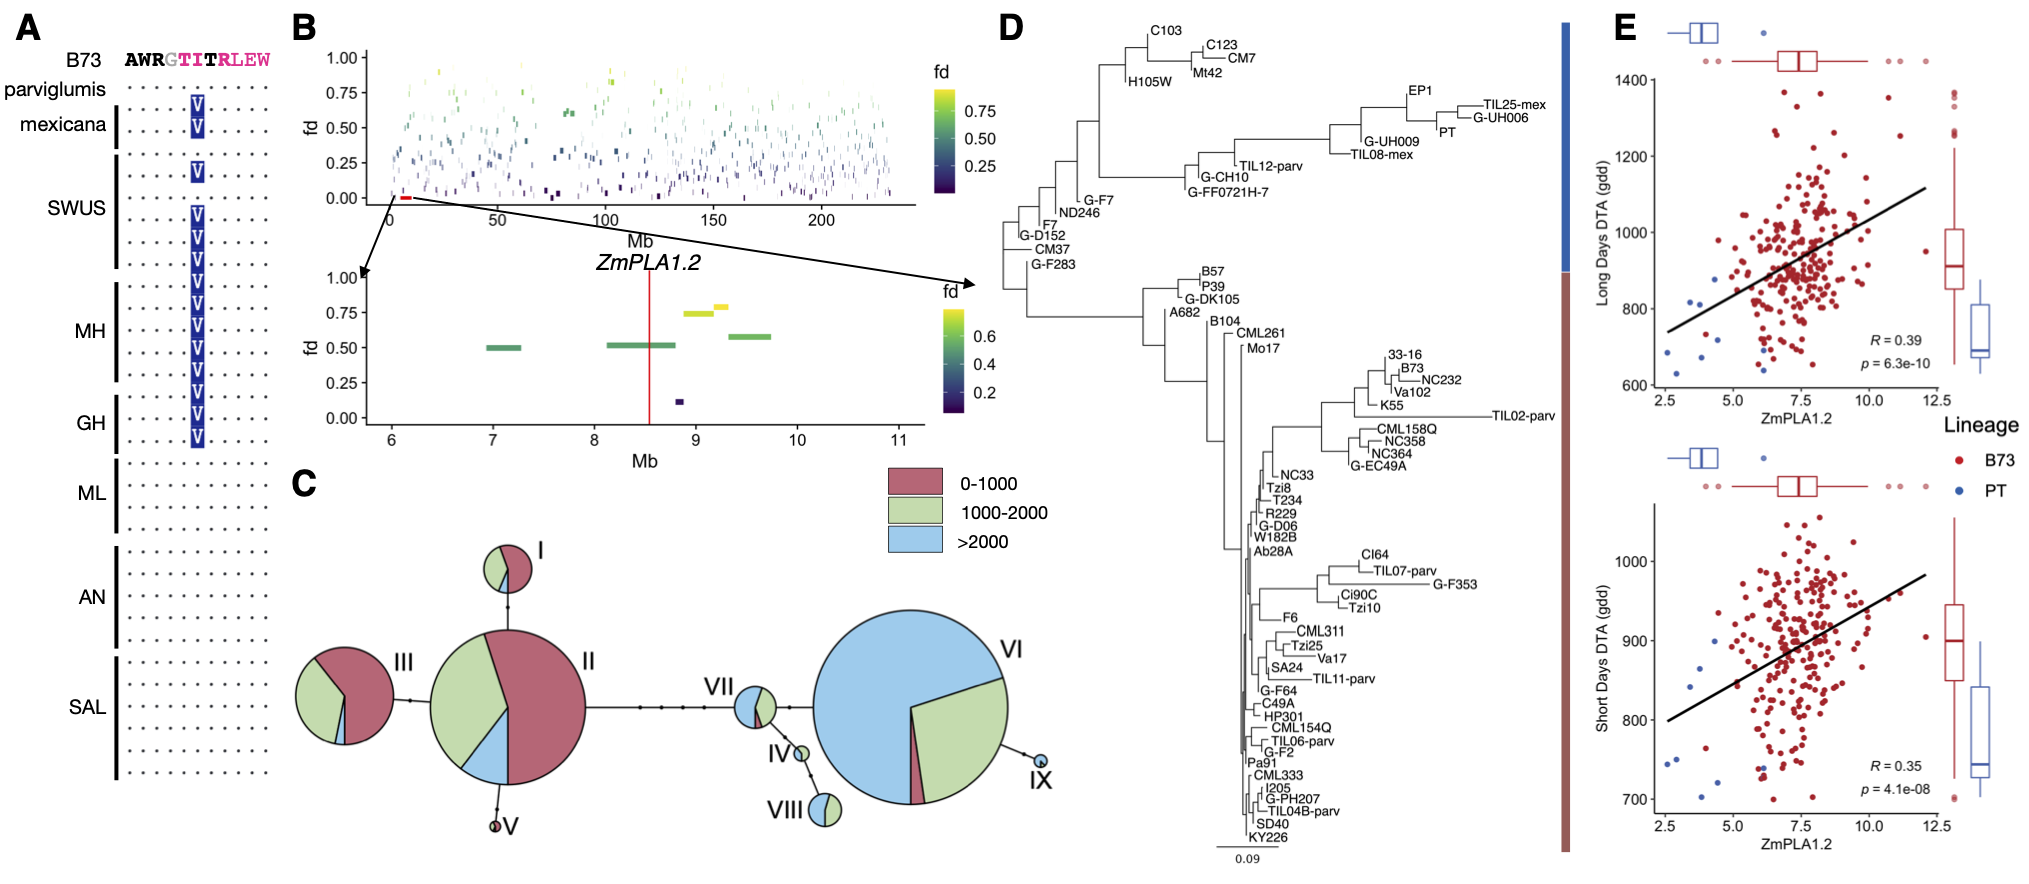
\includegraphics[width=0.4\paperwidth]{Figures/Fig_6.png}
\caption{A)Fitness effects of \textit{ZmPLA1.2-PT}. 
We modeled each trait as a function of \textit{ZmPLA1.2-PT} genotype, trial elevation, and tester line, with controls for main effects and responses to elevation of the genomic background. 
We used BLUPs and GBS data from ~ 2700 landraces from \cite{Gates2019-xu} evaluated in 23 common gardens at different elevations in México. 
Purple lines and ribbons show estimates of the effect of the highland allele of \textit{ZmPLA1.2-PT} as a function of common garden elevation ± 2SE, based on conditional F-tests at the REML solutions of the random effect variance components using the \textit{GridLMM} package \cite{Runcie2019-Gr}. 
Green lines show estimates of the \textit{ZmPLA1.2-PT} effect in a model that additionally included effects of Days-to-Anthesis on the focal trait within each trial.
B) Flowering traits measured in the CRISPR-CAS9 mutant is long day conditions during the Summer of 2020 in Raleigh, NC}. 
\label{Fig6}
\end{center}
\end{figure}

\subsubsection{Association of \textit{ZmPLA1.2} with phosphorus levels}
We measured phosphorus content in flag leaves of highland landraces from México and Perú and B73 grown in control field conditions. Phosphorus levels in highland landraces were higher in B73 (Supplementary Fig \ref{SupFig8}A). 
In México, in geographical locations of accessions of the Seeds dataset, the probability of finding Andosol soils, a type of volcanic soil that has low pH values and low phosphorus availability increased with elevation (Supplementary Fig \ref{SupFig8}B).
It is possible that higher levels of phosphorus in highland landraces might be associated with adaptation to soils with low phosphorus availability. 
To test if \textit{ZmPLA1.2} is associated with phosphorus leaf levels we measured phosphorus content in leaves \textit{ZmPLA1.2} CRISPR-CAS9 mutants but we did not observed any differences (Supplementary Fig \ref{SupFig8}C.) 
PCA analysis of ion levels in mutant and wt plants revealed no differences between the two genotypes (Supplementary Fig \ref{SupFig8}D.) 
\section{Discussion}
\label{sec:discussion}
Understanding the genetic, molecular and  physiological basis of crop species adaptation to different environments and the role that wild relatives has on this processes is relevant to identify favorable genetic variation that can be used to improve modern maize.
Phospholipid metabolism is important for plant adaptation to soils with phosphorus availability \cite{Veneklaas2012-ls, Cruz-Ramirez2004-ib, Lambers2012-an}, low temperature \cite{Degenkolbe2012-wf} and the production of important hormones for plant development and defense such as jasmonic acid. 
%TODO (Allison JA references)
Phospholipids can also be important molecular components of the determination of  \cite{Riedelsheimer2013-bd} probably via interaction with known transcription factors involve in flowering time determination such as flowering locus T \cite{Nakamura2014-qf}. 
Here we show that phospholipid metabolic pathways involved in the synthesis and degradation of phosphatydilcholine species are under strong selection in highland maize landraces and this selection at the genic level is reflected in phosphatydilcholine and lyso-phosphatydilcholine levels of highland landraces from mesomerica grown in highland field conditions leading to a high PC/LPC ratios. 
Using several highland and lowland populations we identified \textit{ZmPLA1.2} and \textit{ZmLPCAT1} as a possible candidates driving this high PC/LPC ratio.
We then identified \textit{ZmPLA1.2} as the major candidate gene explaining a major effect PC/LPC QTL in a B73 x Palomero Toluqueño Backcross Inbred line population. 
The allelic effects of this QTL indicate that the highland PT allele is a loss of function that leads to high PC/LPC ratios by impairing PC to LPC conversion. 
Sequencing of the \textit{ZmPLA1.2-PT} allele identified a SNP in the flap lid domain of the phospholipase that could probably affect substrate specificity and enzymatic activity.
Indeed, a CRISPR KO mutant of \textit{ZmPLA1.2} phenocopied the highland \textit{ZmPLA1.2-PT} allele. 
Evaluation of protein residue variation of the PFAM domain across hundreds of bacteria species further confirmed that the protein residue variation in the flap lid domain is associated with bacterial optimal growth temperature.
We then found that the \textit{ZmPLA1.2-PT} is conserved in Mexican and Guatemalan highland maize and to a lesser extent in Southwest US maize and that this highland allele is the result of highland teosinte \textit{mexicana} into highland maize. 
Moreover, the  \textit{ZxPLA1.2/ZmPLA1.2-PT} haplotype is conserved in Northern US and European Flints and that lower expression of \textit{ZmPLA1.2} is low in this Flint material and is corralated with faster flowering times.
Finally, using phenotypic and genotypic data of thousands of Mexican accessions grown in several common garden trials across Mexico we show that genetic variation of \textit{ZmPLA1.2} shows a strong G x E interaction where the highland allele leads to a delay of flowering time in lowland environments and an accelaration of flowering time in highland environments. 
Other fitness related phenotypes show a similar G X E interaction where the highland \textit{ZmPLA1.2} leads to more fit plants in highland environments and less fit plants in lowland environments. 
This effect was confirmed using a CRISPR mutant of \textit{ZmPLA1.2}.
Our data indicate that \textit{ZmPLA1.2} is a major component of the phpospholipid makepup of maize that can influence several fitness phenotypes important in maize adaptation to low temperatures thorugh physiological and molecular mechanisms that will need to be further investigated.

Given the important role of this environmental factors and plant traits in highland environments, we hypothesized that phospholipid metabolism has been important in the repeated events of maize highland adaptation. 
We studied selection of pathways involved in glycerolipid metabolism (that includes phospholipids but also other non-phosphorus containing polar lipids such as galactolipids) at the genetic pathway level using a Population Branch Excess approach \cite{Pool2017-oa, Wang2020-mp}. 
We found that pathways involved in the synthesis and degradation of phospholipids were repeatedly selected in several highland maize populations of North America, Central America and South America (Figure\ref{Fig1}A-B, Supplementary \ref{SupFig1}A-B). 
These results are similar to other known pathways that are known to be important for highland adaptation such as flowering time \cite{Wang2020-mp}. 
Furthermore, our analysis of the modes of convergence \cite{yeaman2018} indicate that to a certain extent convergence across the different populations is to good extent explained by pleiotropic constraint that limits the number of genes that can determine a phenotype similarly to what we have found in the same populations \cite{Wang2020-mp}.
\textit{ZmLPCAT1} (Zm00001d017584, Lyso-PhosphatidylCholine AcylTransferase 1) and \textit{ZmPLA1.2} (Zm00001d039542, Phospholipase A1 2) showed repeated selection signals of selection in the all four highland populations in the case of \textit{ZmLPCAT1} and in the North American and Guatemalan populations in the case of \textit{ZmPLA1.2}. 
SNPs in the coding regions of \textit{ZmLPCAT1} and \textit{ZmPLA1.2} genes were also strong outliers in the first \textit{pcadapt} principal components (that captures elevation dependent genetic variation) analysis of thousands of accessions across México (Figure \ref{Fig2} and Supplementary \ref{SupFig2}. 
Phospholipid selection in highland maize was also reflected in phospholipid levels and \textit{Qst-Fst} values of phospholipid levels measured from plants of a landrace panel containing highland and lowland landraces grown in a common garden experiments in highland elevations of Mexico and (Figure\ref{Fig1}D-E, Supplementary \ref{SupFig1}C-D). 
\textit{ZmLPCAT1} synthesizes phosphatydilcholine (PC) species via the fusion of a fatty acid and lyso-PhosphatidylCholine (LPC) species (\textit{ZmLPCAT1} while \textit{ZmPLA1.2} hydrolizes PCs into LPCs and fatty acids by acting into the sn1-position. 

In Arabidopsis, \textit{LPCAT1} is involved in the determination of phosphorus leaf content levels under low Zn conditions \cite{Kisko2018-zm}.
In maize a GWAS hit 45 KB upstream of \textit{ZmLPCAT1} for flowering time under low phosphorus conditions further supports the possible role of natural variation of \textit{ZmLPCAT1} in the response to plant to low phosphorus availability. 
In fact, a previous study found that \textit{ZmLPCAT1} showed high \texit {Fst} values when comparing highland and lowland landraces \cite{Takuno2015-uj}.
Natural variation in the maize \textit{ZmPLA1.2} gene or in possible regulatory regions of\textit{ZmPLA1.2} are also associated with lipid content \cite{Riedelsheimer2012-bx} and flowering time \cite{Chen2012-gg, Hung2012-ms} 
In \textit{Tripsacum}, the closest related grass species to \textit{Zea spp} that has adapted to a much more temperate environment than the wild relatives of maize phospholipid synthesis metabolism genes show accelerated rates of evolution \cite{Yan2019-tx} further suggesting that phospholipid metabolism is important for grass adaptation to low temperatures due to latitude or elevation.

%After domestication in the the tropical lowlands of southwest México, maize expanded throughout the Americas and adapted to environmental conditions that are very distinct from the original site of domestication.
%Today maize is  cultivated on all five continents and used for a myriad of culinary and industrial purposes. 
%Understanding the evolutionary, metabolic and physiological mechanisms that enable made to adapt to new environments is relevant both from an agronomical and basic evolutionary genetics point of view.
%In this paper we focused our attention on the role of phospholipid metabolism in the multiple events of maize adaptation to highland environments in the Americas and their

Lipids play an important role in adaptation to new environments. 
As key components of the membranes that maintain cell structure, the fluidity or rigidity a lipid adds to the membrane can be crucial for survival. 
It can be difficult to compare lipid changes across studies, as the time of day the sample is taken, intensity of stress applied, and initial growth environment of the plants can impact the outcome of the lipid analysis \cite{Kenchanmane_Raju2018-nz}. 
Despite these caveats, lipid changes in response to low temperature have been well studied. We observe similar trends between cold-acclimation-imposed lipid changes published in the literature and adaptation-imposed lipid changes in highlands maize. Highland maize shows an increase in PC and decrease of LPC. This trend is matched in Arabidopsis responding to cold acclimation. PC 36:5 and 36:6 increase during cold acclimation, while LPC 18:1 decreases \cite{Welti2002-uk}. PC 36:5 and 36:6 increasing during cold stress also occurs in sorghum \cite{Marla2017-ph}. 
When exploring the lipid changes, they found that maize and sorghum, two relatively cold-sensitive species, displayed increases in desaturation in PC, while tripsacum, the relatively cold-tolerant species, displayed decreases in PC desaturation. The desaturation increase in total PC is matched in a separate sorghum chilling study, as well \cite{Marla2017-ph}. 

Previous studies show that \textit{ZmPLA1.2} in maize is fluctuating with circadian rhythm \cite{Khan2010-iv}. During light hours, \textit{ZmPLA1.2} transcript increases, and during dark hours, it decreases. Changes in phospholipase expression being connected to the clock is not a new phenomenon. Lipids have long been known to fluctuate in response to time of day \cite{Browse1981-vt, Ekman2007-xe}. With specific fatty acids like 16:1, 16:2, and 18:0 highest at the end of the light cycle and 16:3 highest at the end of the dark cycle. Maatta et al 2012 reports that PC in Arabidopsis cycles in this manner \cite{Maatta2012-ip}. PC 34:3, 34:4, 36:5, and 36:6 are all higher at 11 hours into the dark period. Connecting this to the PLA1.2 expression from Khan 2010, it would be plausible that the lack of PLA1.2 would be one component allowing for an increase in PC during the dark. Continuing this trend, LPC 18:1 is also significantly higher at the end of the light period, when PLA1.2 expression is also the highest. 

The increased levels of PC in highland maize may not solely impact membrane function and fluidity, but also may impact flowering time.
Nakamura et al, 2014 showed that PC is intimately tied to flowering as the Arabidopsis protein Flowering locus T (FT) binds to PC in vitro \cite{Nakamura2014-qf}. 
Transgenically increasing PC levels in the shoot apical meristem of Arabidopsis caused a faster flowering time, while lowering them caused flowering delays. 
The ortholog of FT in maize is ZCN8 \cite{Lazakis2011-nq}. ZCN8 underlies a major flowering time QTL and regulatory changes in ZCN8 through various SNPs have allowed maize to adapt its flowering time \cite{Guo2019-pn}.
However, it is not yet known if ZCN8 also has the ability to bind to PC.

\section{Materials and Methods}
\label{sec:materials:methods}
\subsection{Populations used in the analysis } 
Highland and lowland populations used for Population Branch Excess analysis consisted in three to six accessions from each of the highland and lowland populations and have been previously described in \cite{Wang2020-mp, Wang2017-bc}. 

The 120 Landraces from the HiLo Diversity Panel were selected and ordered from the \href{http://mgb.cimmyt.org/gringlobal/search.aspx}{CIMMYT germplasm bank} to maximize a good latitudinal gradient sampling across Mesoamerica and South America. For each highland landrace (>2000 masl) a lowland (<1000 masl) was selected at the same latitude (<0.5$^{\circ}$) to form 60 highland/lowland pairs, 30 in each subcontinent. 
The list of the accessions used is provided in Supplementary file 3.   

B73 x Palomero Toluqueño Backcross Inbred Lines were developed by crossing B73 with a single Palomero Toluqueño plant (Mexi5 accession, CIMMYTMA 2233) that was then backcrossed with B73 once and then selfed five times (BC1S5).  

We used landraces individual accessions genotypic and fitness data from the CIMMYT Seeds of Discovery project (SeeD) \cite{Gates2019-xu} to calculate \textit{pcadapt} \cite{Luu2017-ws} values and GxE effects of \textit{ZmPLA1.2-PT}.

\subsection{Field Experimental Conditions and sampling} 
Two replicas of the Hilo Diversity panel accessions and three replicas B73 x PT BILs were planted in a field located in Metepec, Edo de México, (19°13'28.7"N 99°32'51.6"W) within the Trans-Mexican volcanic belt. 
The field is at 2610 meters above sea level (masl), the range of average monthly temperatures along the year vary from 5 °C to 21.5 °C with an average annual of 13.6 °C.  
Fifty mg of fresh tissue was collected using a leaf puncher from the tip of the second youngest leaf above the last leaf with a fully developed collar around V4-V6 developmental stage. 
Tissue discs were immediately flash frozen in liquid nitrogen. 
All samples were collected in a single day between 10:00 am and 12:00 pm, approximately 3 h after sunrise. 
Samples were transported in dry ice to the lab and stored in -80 C until extraction. 

\subsection{Glycerolipid extraction and UHPLC-QTOF MS/MS lipid profiling} 
Frozen material was homogenized in a tissue grinder Retsch (Haan, Germany) for 40 seconds at a frequency of 30 1/s. After grinding, samples were extracted. 
We performed lipid extraction as reported by Matyash and collaborators \cite{Matyash2008-ue}. 
First, 225 $\mu$L of cold methanol (MeOH), was added to each sample. 
For the blanks, MeOH previously prepared with a Quality Control (QC) mix was added (Supplementary Table XX). Each sample was vortexed for 10 seconds, keeping the rest of materials on ice. 
%TODO: Ruben QC supplementary Table XX
Then 750 $\mu$L of cold methyl tert-butyl ether (MTBE) were added. The MTBE added to the blanks contained 22:1 cholesterol ester as internal standard (Supplementary Table XX). 
Each sample was vortexed for 10 seconds, followed by 6 minutes of shaking at 4°C in the orbital mixer. 
188 $\mu$L of LC/MS grade water at room temperature (RT) was added, and the samples were vortexed for 20 seconds.
We centrifuged the samples for 2 min at 14000 rcf and recovered 700 $\mu$L of supernatant from the upper organic phase. 
We then split the supernatant into two aliquots of 350 $\mu$L, one for lipid profiling and the other for preparation of pools to be used along the lipid profiling. 
Finally, samples were dried with a speed vacuum concentration system.
Dry samples were resuspended in 110 $\mu$L of MeOH-Toluene 90:10 (with the internal standard CUDA, 50 ng/mL). 
Samples were vortexed at low speed for 20 s and then sonicated at RT for 5 min. 
Aliquots of 50 $\mu$L per sample were transferred into an insert within an amber glass vial.
The UHPLC-QTOF MS/MS utilized were Agilent 1290 and Agilent 6530, respectively. 
Before analyzing the samples a new Waters Acquity charged surface hybrid (CSH) C18 2.1x100 mm 1.7 $\mu$m column was set. 
The column was initially purged for 5 min. 
The UHPLC column was coupled to a VanGuard pre-column (Waters Acquity CSH C18 1.7$\mu$m). 
Six “no sample injections” were injected at the beginning of each run to condition the column, followed by ten samples, one pool (made out of the mix of the second aliquot of all the samples contained per UHPLC plate) and one blank.
We injected 1.67 $\mu$L per sample into UHPLC-QTOF MS/MS ESI (+), the running time per sample was 15 min. Mobile phase “A” consisted of 60:40 acetonitrile:water, 10 mM of ammonium formate and 0.1\% formic acid. 
Mobile phase “B” consisted of 90:10 isopropanol:acetonitrile, 10 mM ammonium formate and 0.1\% of formic acid. 
The flow rate was maintained at 0.6 mL/min and the column compartment was maintained at 65° C. Initial conditions were 15\% B; the gradient uniformly increased until reaching 100\%. 
At 12.10 min the mobile phase composition returned to initial conditions.
The mass spectrometer (Q-TOF MS/MS) was operated in positive electrospray ionization mode (ESI), based on the diversity and amount of lipid species identified under ESI (+) and (-) during the lipid profiling optimization (See supplementary Table 3) on Agilent® ultra high performance liquid chromatography and quadrupole time of flight mass spectrometry (UHPLC-QTOF MS). 
For this optimization we used 8 samples of B73, 8 samples of PT and 10 samples of a recombinant inbred line population (BILs) generated by crossing B73 and PT, only MS1 data was acquired. 
The same samples were utilized for both ESI modes. 
Under positive mode 24 lipids were identified, having two cholesterol esters (CE), 3 diacylglycerols (DAG), 2 lysophosphatidylcholines (LPC), 10 phosphatidylcholines (PC), 1 phosphoethanolamine (PE) and 6 triacylglycerols (TAG). 
While under negative mode we identified 16 lipids, of which, 14 were fatty acids (FA) and 2 were PC species. 
For the source parameters, ESI gas temperature was set at 325 °C, nebulizer pressure of 35 psig, gas flow of 11L/min, capillary voltage at 3500 V, nozzle voltage at 1000V, MS TOF fragmentor and skimmer at 120 and 65 V, respectively.
Under the acquisition parameters a mass range between 60 and 1700 m/z was set. As for reference mass parameters, a detection window of 100 ppm and a minimum height of 1000 counts were set. 
%CRISPR-CAS9  methods

\subsection{Glycerolipid data processing}
We performed a retention time (rt) correction of the acquired data using Agilent MassHunter Qualitative Analysis® B.06.00 version and Microsoft Excel. 
To extract ion chromatograms (EICs) of the internal standards within the run we used Agilent MassHunter Qualitative Analysis.
We identified the time of the highest intensity point of each EIC, which then was used as the current retention time of the experiment. 
In Microsoft Excel, using the method retention time for internal standards and the current rt, a polynomial regression was obtained and used for calculating new retention times for 501 lipids listed in a MS1 m/z-rt library from Dr. Oliver Fiehn laboratory (See Supplementary Table 2).
In MSDIAL \cite{Tsugawa2015-kh}, identification of lipids is based on two approaches: the MSP file and MS/MS identification setting included in MSDIAL and the use of a post identification file containing accurate m/z and rt for a list of lipids. In this study we used both identification approaches. 
The MSP file and MS/MS identification setting has a total of 51 lipid classes, under positive ion mode, that can be selected for identification. 
The post identification file that we used was the retention time-corrected MS1-MS2 mz-rt lipid library that we explained before. 
We used MSDIAL \cite{Tsugawa2015-kh} version 3.40. To use MSDIAL, the raw data was converted from .d to .abf format with Reifycs Abf converter (https://www.reifycs.com/AbfConverter/). 
The MSDIAL alignment results were filtered out based on whether compounds intensity was ten times above blank intensity. 
Then, filtered data was normalized using Systematic Error Removal using Random Forest (SERRF) \cite{Fan2019}, this normalization is based on the quality-control pool samples used along the study. Normalized features were filtered out considering a coefficient of variation (CV) equal or less than 30\% along the pools. 
To curate the data for duplicate features, isotopes and ion-adducts we utilized MS-FLO \cite{DeFelice2017-ms}.
Curated data was also normalized using sum known metabolite signal (mTIC). 
After data processing and normalization, lipid intensities were used for further analysis.
%CRISPR-CAS9  methods

\subsection{Glycerolipid pathways selection}
We compiled a list of genes pertinent to glycerolipid metabolism starting with a search of all genes belonging to the \textit{Zea mays} 'Glycerophospholipid metabolism' and 'Glycerolipid metabolism' KEGG pathways \cite{kanehisa2019} (map identifiers: zma00564 and zma00561). 
With the NCBI Entrez gene identifiers in KEGG we retrieved the AGPv4 transcript identifiers used in Corncyc 8.0 \cite{portwood2019, walsh2016} from an id cross reference file found in MaizeGDB (\href{https://www.maizegdb.org/search/gene/download_gene_xrefs.php?relative=v4}) \cite{portwood2019}.
This resulted in a list of 300 genes comprising 51 Corncyc pathways. 
Then we discarded Corncyc pathways  tangentially connected to the KEGG glycerolipid metabolism list (sharing just one enzyme with the initial KEGG list) or that we judged to belong to different biological processes (e.g 'long chain fatty acid synthesis','anthocyanin biosynthesis'). 
Finally, we added manually the 'phosphatidylcholine biosynthesis V' pathway that was missing. 
The list of 30 selected Corncyc pathways included genes outside the initial KEGG search results and raised the number of genes to 557. 
In addition to this, 37 genes were found to have an enzymatic activity related to phospholipid metabolism but not placed into any particular pathway, i.e orphan enzymes, consisting mostly of alcohol dehydrogenases. 
Sixteen additional genes found in KEGG were not annotated at all in Corncyc probably due to differences between AGPv4 and RefSeq pseudogene annotation of the maize genome. 
The list of all possible candidates coming either from KEGG or Corncyc that were orphan enzymes or were unannotated in Corncyc amounted to 594 genes (Supplementary File 1). 
This process is documented in the \verb|0_get_glycerolipid_genes.R| script of the \verb|pgplipid| R package accompanying this paper \cite{fausto_rodriguez_zapata_2020_4323410}.

\subsection{Population Branch Excess Analysis}
Population Branch Excess quantifies changes in allele frequencies in focal populations relative to two independent “outgroup” populations.
We used \textit{Zea mays spp. parviglumis} as one of the outgroup populations for all four highland groups.  
The other outgroup was  Mexican lowlands  in the case of southwest US , Mexican highlands and Guatemalan highlands; and South American lowlands in the case of the Andes population. 
After calculating genome wide PBE scores for the 4 populations (described in detail in \cite{Wang2020-mp}), we tested for selection outliers SNPs in the 594 phosphoglycerolipid candidates and the 30 Corncyc pathways (556 genes).
We first defined a PBE outlier SNPs as the top 5\% of the PBE score distribution, this fraction corresponds to approximately 50000 out of ~1 million genotyped SNPs in each population. 
We defined a gene as a PBE outlier if it contained an outlier SNP within the coding sequence or 10 Kbp upstream/downstream  \cite{Wang2020-mp}. 
Then we tested for over-representation of genes selected in particular subsets of populations using Fisher's exact test using the 32283 protein genes from the maize genome (Supplemental Figure 1a) \cite{wang2015a} as background. 
For each pathway, we first selected all SNPs that include CDS regions and 10Kb upstream and downstream of the gene and we calculated the mean pathway PBE score. 
We then constructed a null distribution by drawing 10000 samples without replacement of $n$ SNPs from those found within or around 10Kb upstream and downstream of all protein coding genes and we obtained the mean PBE for this null distribution. 
%For each pathway, the heat map shows p-values corresponding to the probability of sampling from the null distribution a set of $n$ SNPs with the observed glycerolipid pathway mean PBE score or higher.
With the set of PBE ouliers for glycerolipid metabolism in the 4 populations we tested for evidence of physiological or pleiotropic constraint using the $C_\chi^2$ statistic \cite{yeaman2018}. 

\subsection{\textit{$Q_{ST}$-$F_{ST}$} analysis of glycerolipid data}
Quantitative trait divergence ($Q_{ST}$) was contrasted to the distribution of $F_{ST}$ for neutral genetic markers \cite{whitlock2008evolutionary}.
Highland/Lowland contrasts were considered separately for Mesoamerica and South America.

A linear mixed effects model (R package lmer, function lmer) was used to partition phenotypic variance between population pairs (Mesoamerica/South America, all highland/all lowland, Mesoamerican highland/Mesoamerican lowland, South American highland/South American lowland).

\begin{center}

${ TRAIT \sim 1 + (1|POPULATION) + }$\\
${(1|GARDEN/BLOCK) + (1|BATCH)}$

\end{center}

Within-population and between-population variances were calculated with the R function VarCorr (R package \texttt{lme4}, \citealp{bates2014lme4}), and were used to calculate $Q_{ST}$ following the equation below:

\begin{center}
$Q_{ST}$ = \(\sigma^{2}_{GB}/(\sigma^{2}_{GB}+2\sigma^{2}_{GW})\)
\end{center}

\noindent in which $\sigma^{2}_{GB}$ and $\sigma^{2}_{GB}$ are the between- and within-population genetic variance components, respectively \cite{Leinonen2013-ic}.

Pairwise $F_{ST}$ was calculated with the R function fst.each.snp.hudson (R package \textit{dartR}, \citealp{gruber2018dartr}).
$Q_{ST}$ values were considered significantly high or low if they were greater or less than than two standard deviations from the mean $F_{ST}$.
\subsection{\textit{pcadapt} analysis of biological adaptation in Mexican landraces}

In order to conduct genome scans for signatures of adaptation we used the pcadapt \cite{Luu2017-ws} package.
\textit{pcadapt} identifies adaptive loci by measuring how strongly loci are contributing to patterns of differentiation between major axes of genetic variation.
Under simple models the principal component based models of pcadapt capture major patterns of $F_{ST}$ outlier tests but are conducted in a way that does not require population delimitation \cite{duforet2014genome}.
%Population delimitation is difficult in maize landraces which, in general, contain low levels of differentiation as well as complicated demographies based upon long distance migration alleles owing efforts by farmers to maintain genetic diversity and test for new adaptive genetic combinations.
As the genome scan comparison requires a focal SNP to be compared to the first K principal components of the genotype data, it can be biased by large regions of low recombination that drive the major axes of variation in the principal components.
Thus, when SNPs from these low recombination regions are compared against principal components driven by linked loci spurious signals may arise.
To prevent this bias from occurring, we used custom scripts to calculate the principal component step separately based upon all the chromosomes except for the chromosome of the focal SNPs being tested.
The genotype data we used for this analysis was GBS data from roughly 2,000 landraces of Mexican origin collected by CIMMYT (www.cimmyt.org) as part of the SeeDs of discovery initiative (https://www.cimmyt.org/projects/seeds-of-discovery-seed/).
From this, we calculated the strength of association between each SNP and the first five principal components (excluding the chromosome of the focal SNP) using the communality statistic as implemented in \textit{pcadapt} version 3.0.4.

\subsection{QTL analysis of phospholipid levels}
We analyzed glycerophospholipid QTLs in a mapping population of 57 BILs (BC1S5) from the cross B73 x (PT).
These BILs were grown in a highland site in Metepec, Edo de Mexico at 2600 masl during the Summer of 2016 and in Puerto Vallarta, Jalisco at 50 masl during the Winter of 2016/17. 
We analyzed the samples using UHPLC-QTOF, as above, and 67 leaf lipid species were identified.
For QTL analysis we calculated the mean across all fields of individual lipid mass signal. 
We also used as phenotypes the sum total of the following lipid classes: diacylglycerol, triacylglycerol, phosphatidylcholine and  lysophosphatidylcholine.  
Furthermore,  we also included the log base 10 transformed ratios of LPCs/PCs and the ratios of their individual species. 
We did a simple single marker analysis  with ``scanone`` using Haley-Knott  regression, and assessed the QTL significance with 1000 permutations.

\subsection{CRISPR-CAS9 editing of \textit{ZmPLA1.2} and analysis of the effect of \textit{Zmpla1.2\textsuperscript{CR}} mutant on flowering time}
CRISPR/Cas9 was used to create a \textit{ZmPLA1.2} gene knockout through agrobacterium mediated transformation of background line B104 \cite{Wu2020-nq, Char2017-uk}. 
Guide RNA was designed as described in \cite{Brazelton2015-co} for the B73 reference genome v4. 
B104 and B73 sequence for \textit{ZmPLA1.2} were identical. 
gRNA cassette was cloned into pGW-Cas9 using Gateway cloning. 
Two plants from the T0 transgenic event were identified through genomic PCR amplification and Sanger sequencing and were self-pollinated. 
Several T1 plants containing the \textit{ZmPLA1.2\textsuperscript{CR}} event were selected and planted for lipid analysis in greenhouses at the North Carolina State University during the 2020 Spring, genotyped using forward primer CAGTTCTCATCCCATGCACG and reverse primer CCTGATGAGAGCTGAGGTCC and  self-pollinated. 
Cas9 positivity was tested for using 0.05\% Glufosinate ammonium contained in Liberty herbicide. 
T2 seeds from CAS9 free T1 plants were collected and used for flowering time analysis in  Clayton, NC during the 2020 Summer. 
\subsection{Subcellular localization of \textit{ZmPLA1.2}}
\subsection{Sanger sequencing of \textit{ZmPLA1.2} in BILs homozyogous at the \textit{qPC/LPC3@8.5} locus}

\subsection{Expression analysis of \textit{ZmPLA1.2} and \textit{ZmLPCAT1} in B73, PT and B73xPT F1s in conditions simulating highland environments}

\subsection{Bacterial optimal growth temperature association with ZmPLA1.2 flap-lid domain allelic variation}
The maize \textit{ZmPLA1.2} protein sequence was compared to prokaryotes with the same sequence to determine whether the identified residue change in maize and accompanying association with low temperature survival was consistent with observations in other organisms. 
Pfam domain PF01764 was identified in the B73 protein sequence using the HMMER3 web server, and 982 observations of the PF01764 Pfam domain were identified in 719 prokaryote species using PfamScan \cite{Potter2018-tk, El-Gebali2019-pw}. 
The optimal growth temperature of these species was predicted using tRNA sequences as in \cite{Cimen2020-dm}. 
Maize and prokaryote PF01764 domain sequences were aligned with hmmalign from the hmmer3 package \cite{Eddy2011-pd}, and the aligned Pfam sequences were recoded to reflect nine amino acid physicochemical properties \cite{Li2016-ut}. 
Sequences were filtered to remove gaps in the domain alignment and observations with only partial domain sequences, then clustered based on sequence similarity, resulting in two clusters of observations within the domain. 
For each cluster, positions in the filtered alignment were associated with prokaryote optimal growth temperatures using a linear regression with all 9 amino acid physicochemical properties. 
Seventeen sites in and around the flap-lid region of the protein passed a 10\% FDR significance threshold, including the single residue change p.Ile211Val previously identified in \textit{ZmPLA1.2-PT}. 
Welch’s two-sided t-test was used to compare the optimal growth temperatures of prokaryote species with the \textit{ZmPLA1.2-B73} allele to the optimal growth temperatures of prokaryote species with the \textit{ZmPLA1.2-B73} allele at this site.

\subsection{Nucleotide Diversity of \textit{ZmPLA1.2} }
We estimated nucleotide diversity for the promoter and coding regions of \textit{ZmPLA1.2} using WGS data from highland and lowland accessions from México and South America obtained from \cite{Wang2017-bc} and the R package PopGenome \cite{Pfeifer2014-bg}. 
FASTA files were partitioned into 4 populations by origin  supplemental for accessions included) and then subset into coding and promoter regions, which was defined as 3Kb upstream of the cds. 
Data were imported into PopGenome using the option include.unknown=FALSE in order to prevent bias by excluding missing and ambiguous nucleotide data.
Pi was measured separately within each population and averaged by the number of sites in the coding and promoter regions. 

\subsection{Teosinte \textit{mexicana} introgression in highland maize}
To evaluate if the \textit{ZmPLA1.2-PT} allele was the result of standing variation from teosinte \textit{parviglumis} or introgression from \textit{mexicana} we used Patterson's \textit{D} statistic and genome-wide $f_{d}$ to calculate ABBA-BABA patterns. 
The data was obtained from \cite{Gonzalez-Segovia2019-jy}. 
The material used in \cite{Gonzalez-Segovia2019-jy} included whole genome sequence data from three highland outbred individuals: two Palomero Toluqueño and one Mushito de Michoacán; three lowland landraces: Nal Tel (RIMMA0703) and Zapalote Chico (RIMMA0733) obtained from \cite{Wang2017-bc} and  BKN022 from \cite{Bukowski2017-ng}; two \textit{mexicana} inbreds: TIL08 and TIL25; three \textit{parviglumis} inbreds: TIL01, TIL05, TIL10 and \textit{Tripsacum} TDD39103 \cite{Bukowski2017-ng} as an outlier. 

\subsection{Haplotype network analysis of \textit{ZmPLA1.2} in Mexican maize landraces and teosintes.}
We extracted SNP genotypes for \textit{ZmPLA1.2} from the TIL teosinte accessions HapMap 3 imputed data \cite{Bukowski2017-ng} and the 3700 Mexican landraces in the SEEDs dataset. 
With the set of 1160 accessions that were homozygous at all sites in this genomic region we calcultaed an haplotype network depicting the minimal spanning tree for haplotypes covering 90\% of the input accessions with the R package \code{pegas} \cite{paradis2010}, and haplotype frequencies for three elevation classes in the landraces (0-1000,1000-2000, >3000 masl).

\subsection{Phylogenetic analysis of\textit{ZmPLA1.2} in maize inbreds and teosintes.}
Using v3 of B73 genome, \textit{ZmPLA1.2} SNPs were obtained from the 282-panel, the German inbreds and teosinte TIL inbreds from HapMap 3 \cite{Bukowski2017-ng}. 
SNPs were aligned using Geneious2020.0.5 and a neighbor-joining phylogenetic tree was generated. 
To facilitate visualization and interpretation of the tree we condensed tree branches from lines with identical haplotypes and from similar geographic locations. 
The full tree is available as Supplementary file 4. 

\subsection{Expression analysis of candidate genes and association with flowering traits in the 282 panel}
We used gene expression RNA-Seq data obtained from the 282 panel at different developmental stages \cite{Kremling2018-gn} and BLUP values of several flowering and photoperiod sensitiviy traits \cite{Hung2012-ms} to study the correlation of \textit{ZmPLA1.2} expression values in the 282 panel with flowering time traits.  

\subsection{Association of \textit{ZmPLA1.2} with agronomic traits}
We re-analyzed phenotypic data from the F1 Association Mapping (FOAM) panel of Romero-Navarro \textit{et al} \cite{Romero_Navarro2017-cn} and Gates \textit{et al} \cite{Gates2019-xu} to more fully characterize associations signatures of \textit{ZmPLA1.2}. 
Full descriptions of this experiment and data access are described in those references. 
We downloaded BLUPs for each trait and line from Germinate 3, and subseted to only those lines with GBS genotype data from México. 
We fit a similar model to the GWAS model used by Gates \textit{et al} \cite{Gates2019-xu} to estimate the effect of the \textit{ZmPLA1.2-PT} allele on the trait's intercept and slope on trial elevation, accounting for effects of tester ID in each field and genetic background and family effects on the trait intercept and slope using four independent random effects. 
We implemented this model in the \textit{R} package \textit{GridLMM} \cite{Runcie2019-Gr}. 
We extracted effect sizes and covariances conditional on the REML variance component estimates and used these to calculate standard errors for the total \textit{ZmPLA1.2-PT} effect as a function of elevation. 
To test whether the phenotypic effects of \textit{ZmPLA1.2-PT} on yield components could be explained as indirect effects via flowering time, we additionally re-fit each model using Days-To-Anthesis as a covariate with an independent effect in each trial.

\subsection{Effect of \textit{Zmpla1.2\textsuperscript{CR}} mutant on flowering time}
Seeds of T2 CAS9-free plants were grown in isolation during the 2020 Summer in Clayton, NC. Female (Days to Silking) and male (Days to Anthesis) flowering time were calculated from the day of planting until the first silks and anther pollen shed could be observed in each individual plant. 
Plants homozygous \textit{Zmpla1.2\textsuperscript{CR}} and WT derived from the same T1 families were planted for this experiment. 
Effect size analysis was performed using the dabestR package \cite{Ho2019-yl}.

\subsection{Phosphorus analysis and phosphorus soil availability data}
We analyzed phosphorus content in B73 and 5 Mexican  and 5 Peruvian highland landraces (Supplementary file 1) grown in control field conditions in the 2018 Puerto Vallarta, México, Winter nursery. 
Samples were analyzed using ICP-MS according to \cite{Baxter2014-ch}. 
Frequency of Andosol soils at different elevations was calculated using the soilP package \cite{Rodriguez-Zapata2018-vz}.
Phosphorus content in flag leaves of the the same \textit{Zmpla1.2\textsuperscript{CR}} and WT mutants used for the flowering time experiment were analyzed using ICP-OES at the North Carolina Department of Agriculture.   

\section{Acknowledgments}
\label{sec:acknowledgments}

\bibliography{bibliography}

\section*{Supplemental Tables and Figures}

\renewcommand{\thefigure}{S\arabic{figure}}
\renewcommand{\thetable}{S\arabic{table}}%
\linenumbers

\setcounter{figure}{0}
\setcounter{table}{0}
\begin{figure*}[t]
\begin{center}
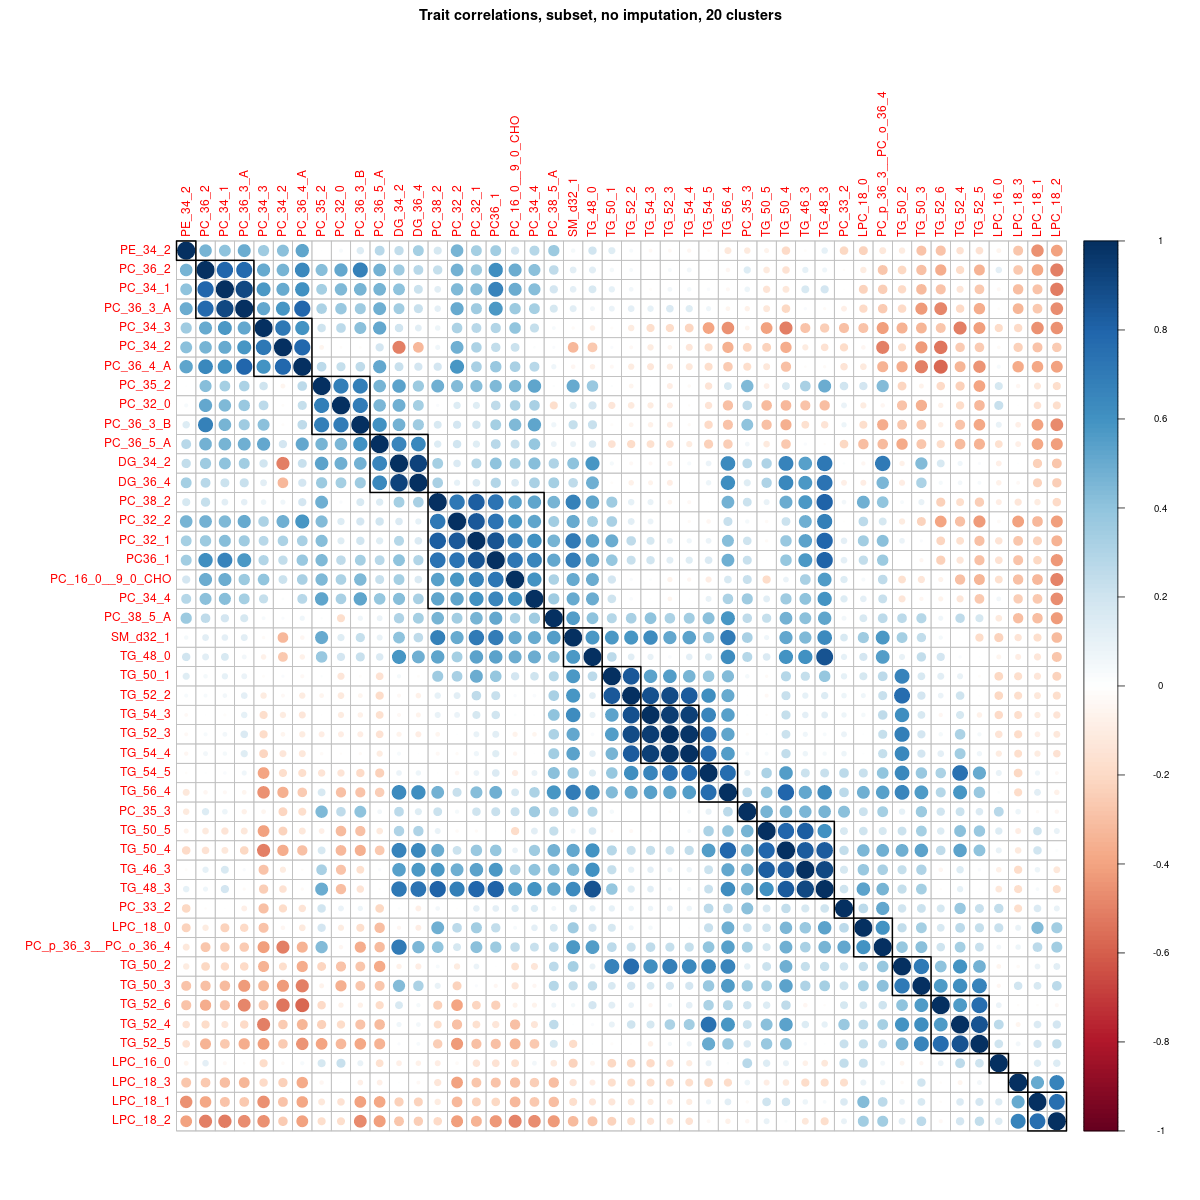
\includegraphics[width=0.8\paperwidth]{Sup_Figures/Sup_Fig_1.png}
\caption{A) Population Branch Excess Analysis of glycerolipid pathway genes.
A)From the initial set of 211 genes we used 186 genes with 6219 non redundant SNPs and 683162 non redundant SNPs for the SW US group; 186 genes with 6106 non redundant SNPs and 664555 non redundant SNPs for the Mexican Highland group; 185 genes with 5912 non redundant SNPs and 641186 non redundant SNPs for the Guatemalan Highlands group; and 184 genes with 5698 non redundant SNPs and 614783 non redundant SNPs for the Andes group.
B) Example of pathway 7416 (phospholipid remodeling) PBE values (red lines) for each highland population and genome wide PBE distributions (black histograms). 
\textit{$Q_{ST}$-$F_{ST}$} analysis of glycerolipid compounds between highland and lowland landraces from MesoAmerica (C) and South America (D).
Samples for Dart-Seq genotyping were taken from the same plants that were grown in the common garden experiment shown in Figure 1D-F and that were used for glycerolipid analysis. 
}
\label{SupFig1}
\end{center}
\end{figure*} 

\begin{figure*}[t]
\begin{center}
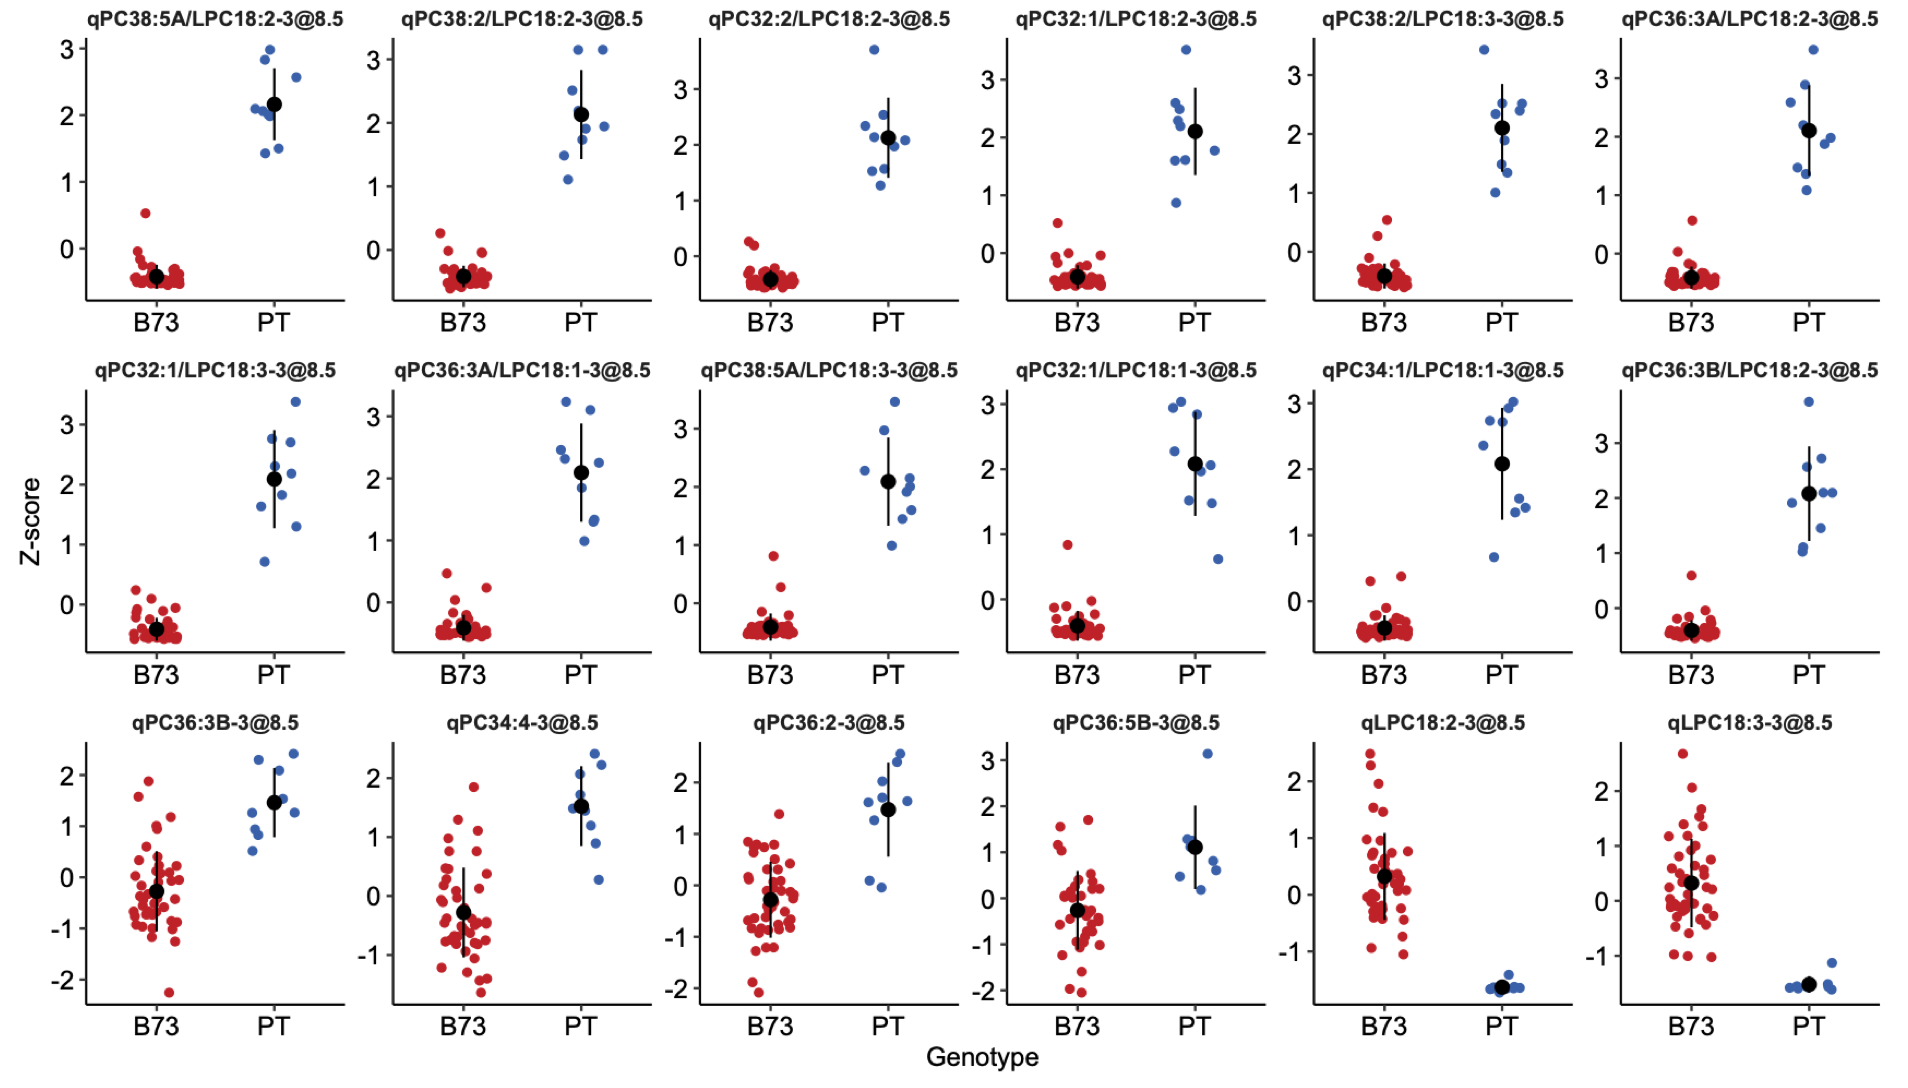
\includegraphics[width=0.8\paperwidth]{Sup_Figures/Sup_Fig_2.png}
\caption{\textit{Pcadapt} analysis of Mexican landraces. We used GBS data from the Mexican landraces of the SEEDs dataset \cite{Romero_Navarro2017-cn} and run a \textit{pcadat} analysis \cite{Luu2017-ws} that identified (A) elevation as the major driver of population differentiation polarizing PC1.  
B) Genome wide analysis of \textit{Pcadapt} PC1 outliers. 
}
\label{SupFig2}
\end{center}
\end{figure*} 

\begin{figure*}[t]
\begin{center}
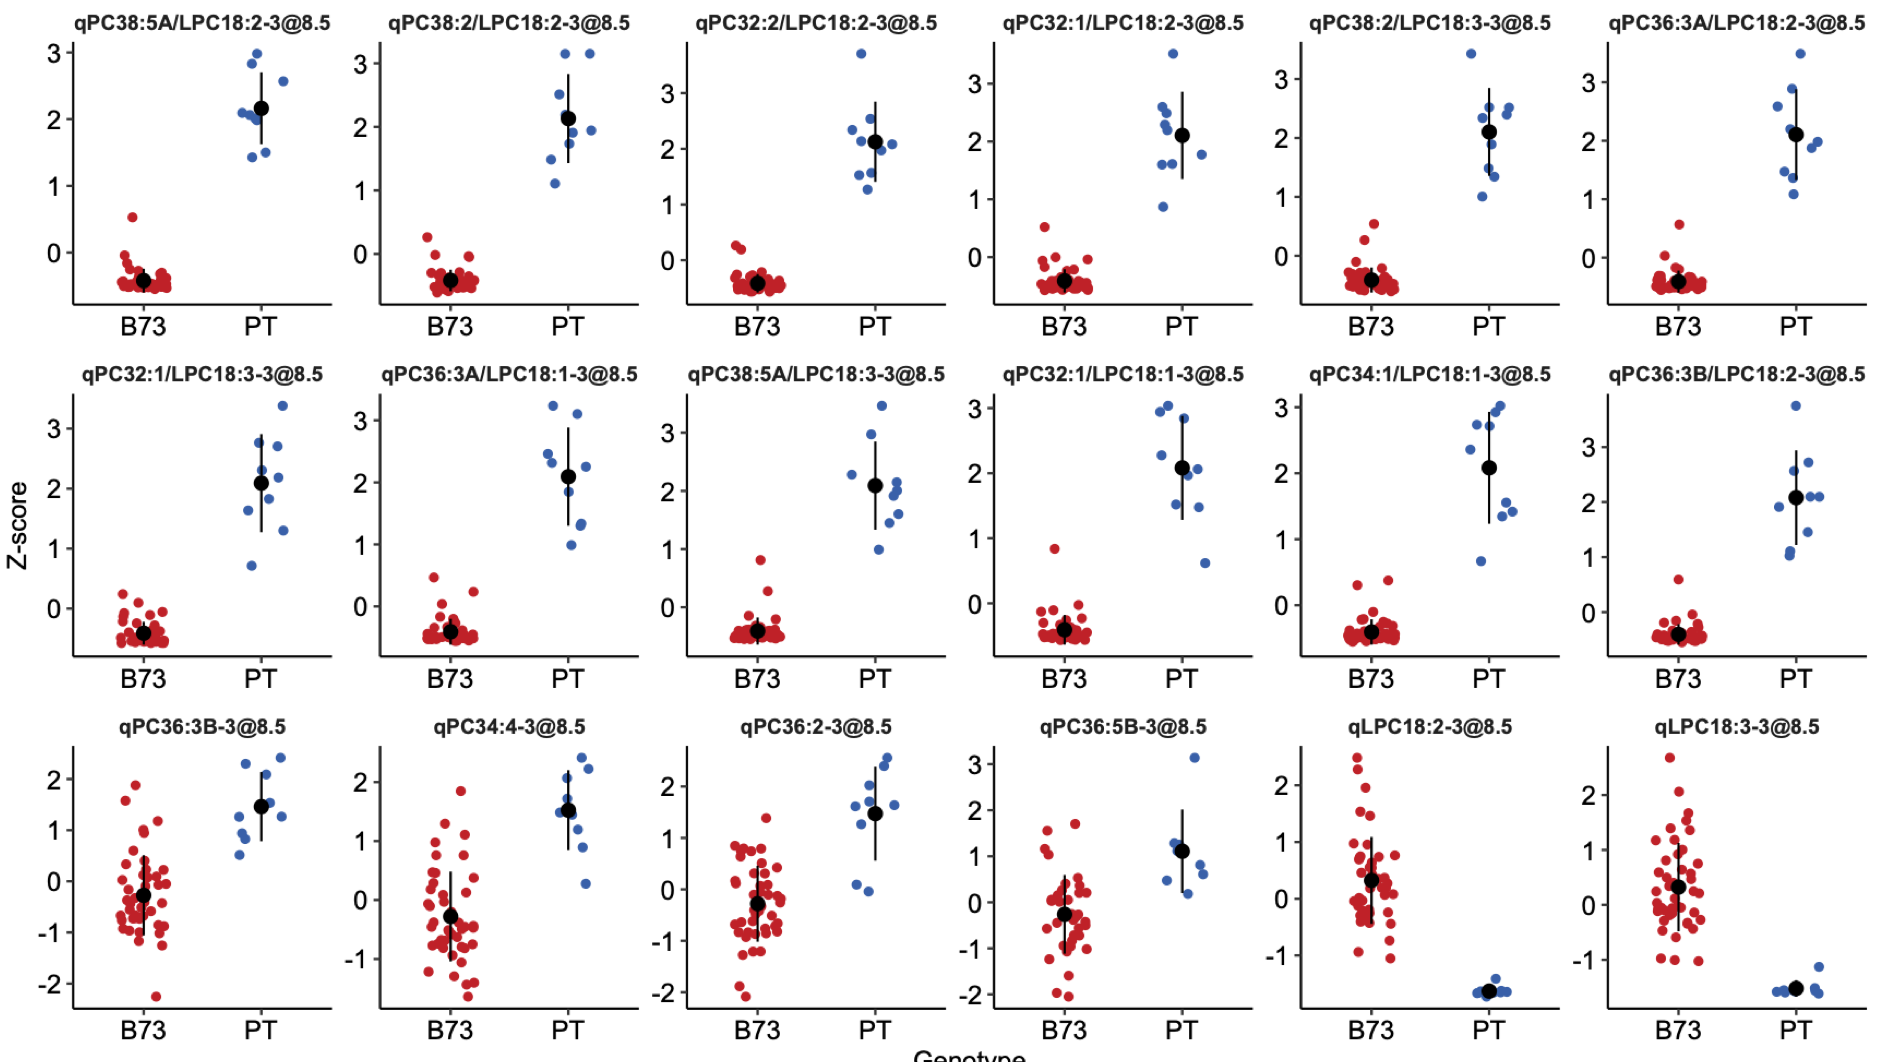
\includegraphics[width=0.8\paperwidth]{Sup_Figures/Sup_Fig_3.png}
\caption{A) Genomic Location of genes coding for enzymes predicted Phospholipase A1 activity. 
B) Site of action of the different types of phospholipases.
C) Subcellular localization of \textit{ZmPLA1.2}.
D) B73 expression levels of genes coding for enzymes with predicted Phospholipase A1 activity across different tissues. \textit{ZmPLA1.2} is indicated in blue. 
E) \textit{ZmPLA1.2} expression levels of temperate inbreds B73, Mo17, Oh43, and Ph207 under control, control and heat stress. Values taken from \cite{Waters2017-nat}. 
}
\label{SupFig4}
\end{center}
\end{figure*}  

\begin{figure*}[t]
\begin{center}
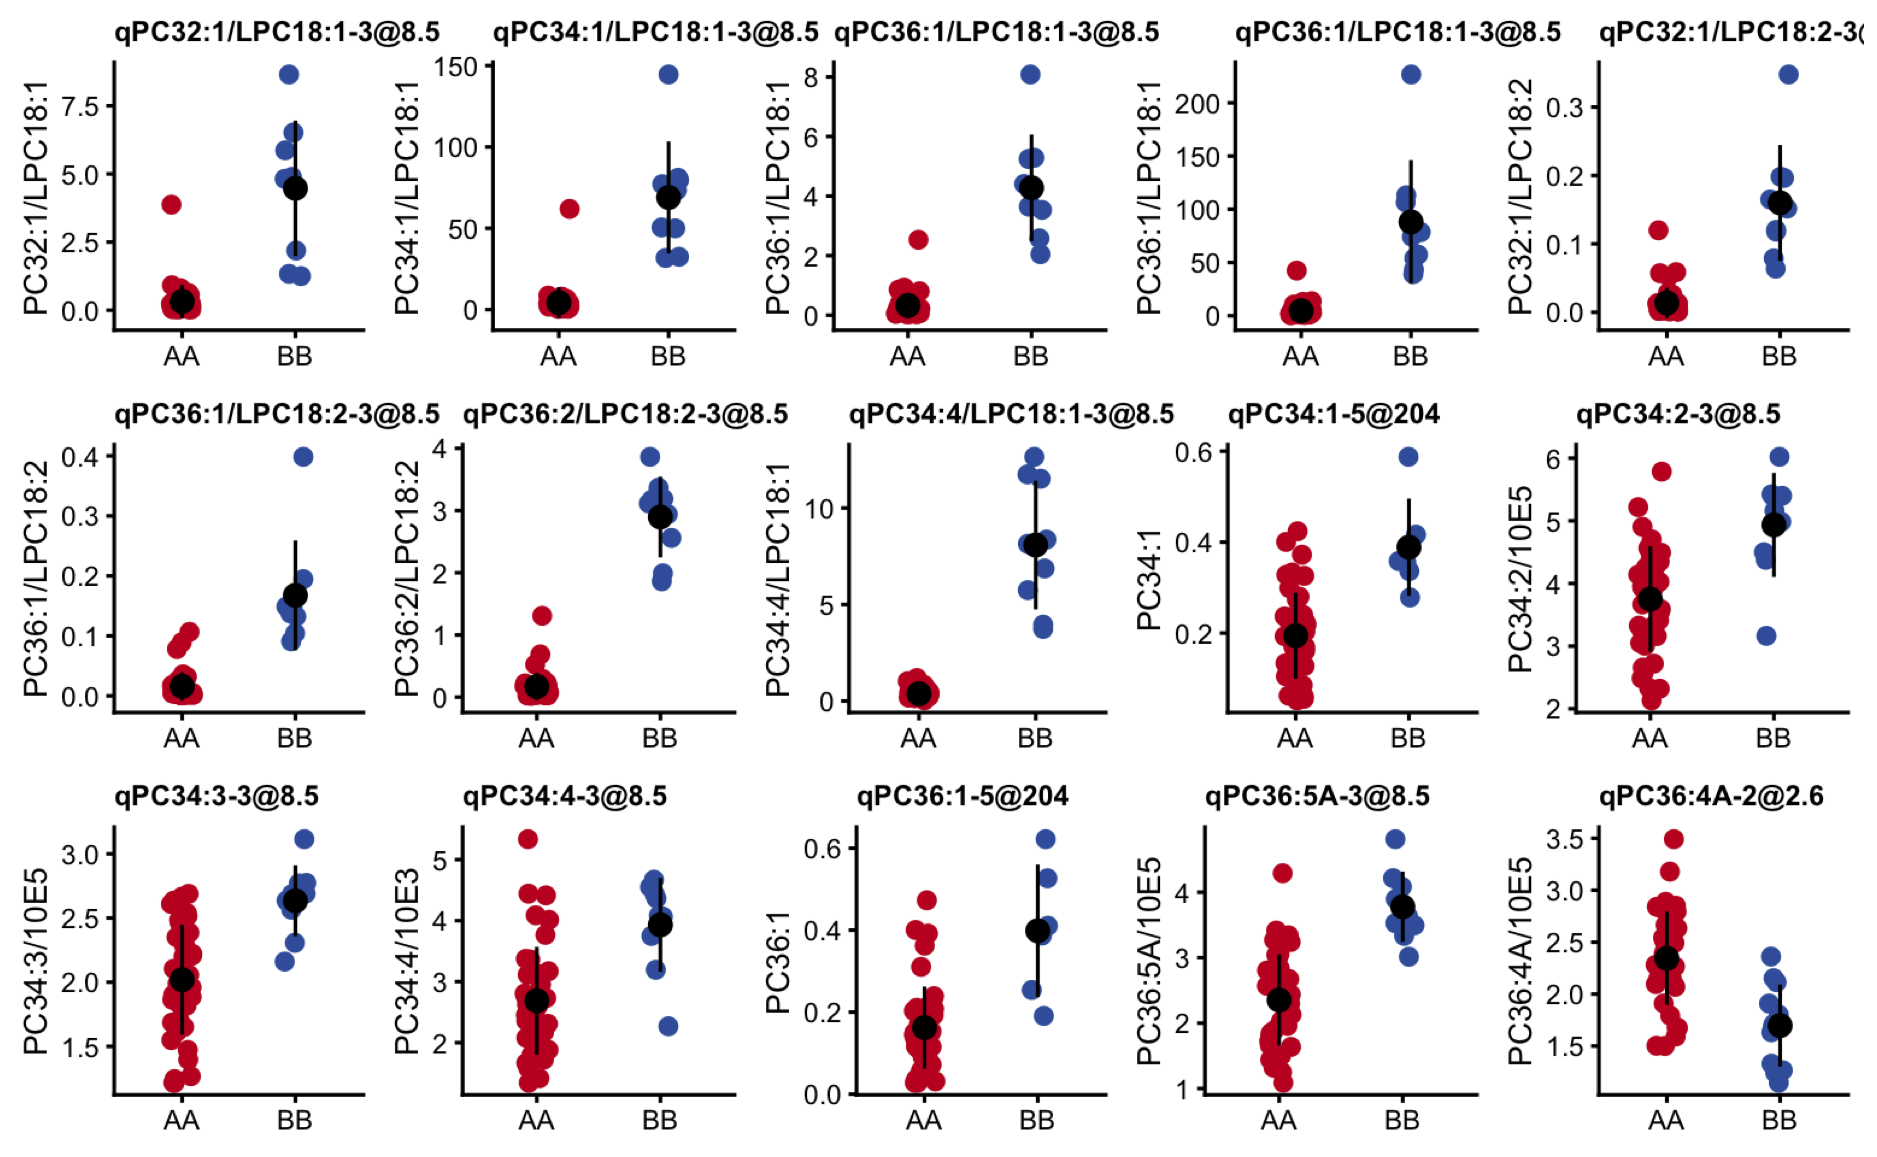
\includegraphics[width=0.8\paperwidth]{Sup_Figures/Sup_Fig_4.png}
\caption{A) Effect sizes of several individual PC, LPC, and PC/LPC QTL peaks used to calculate the Orr test of selection.  
}
\label{SupFig3}
\end{center}
\end{figure*} 

\begin{figure*}[t]
\begin{center}
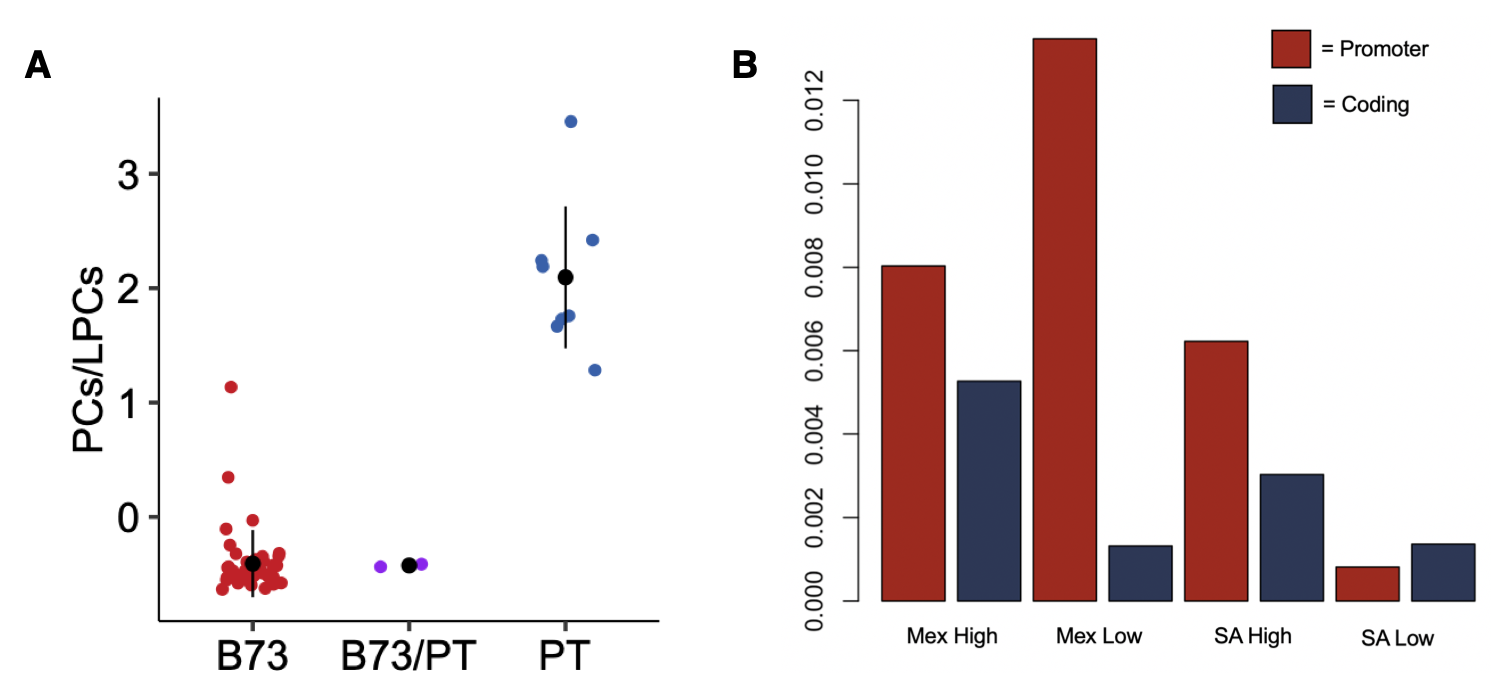
\includegraphics[width=0.8\paperwidth]{Sup_Figures/Sup_Fig_5.png}
\caption{A)Effect sizes of PC/LPC levels at BILs homozyzogous B73, PT and heterozygous qPC/LPC3@8.5.
B) Flap lid domain and catalytic triad \textit{ZmPLA1.2} protein alignment from several plant species. 
C) Nucleotidy diversity analysis of the promoter and CDS region of \textit{ZmPLA1.2} using whole genome sequencing data of highland and lowland landraces México and South American obtainedfrom \cite{Wang2017-bc}
}
\label{SupFig6}
\end{center}
\end{figure*} 

\begin{figure*}[t]
\begin{center}
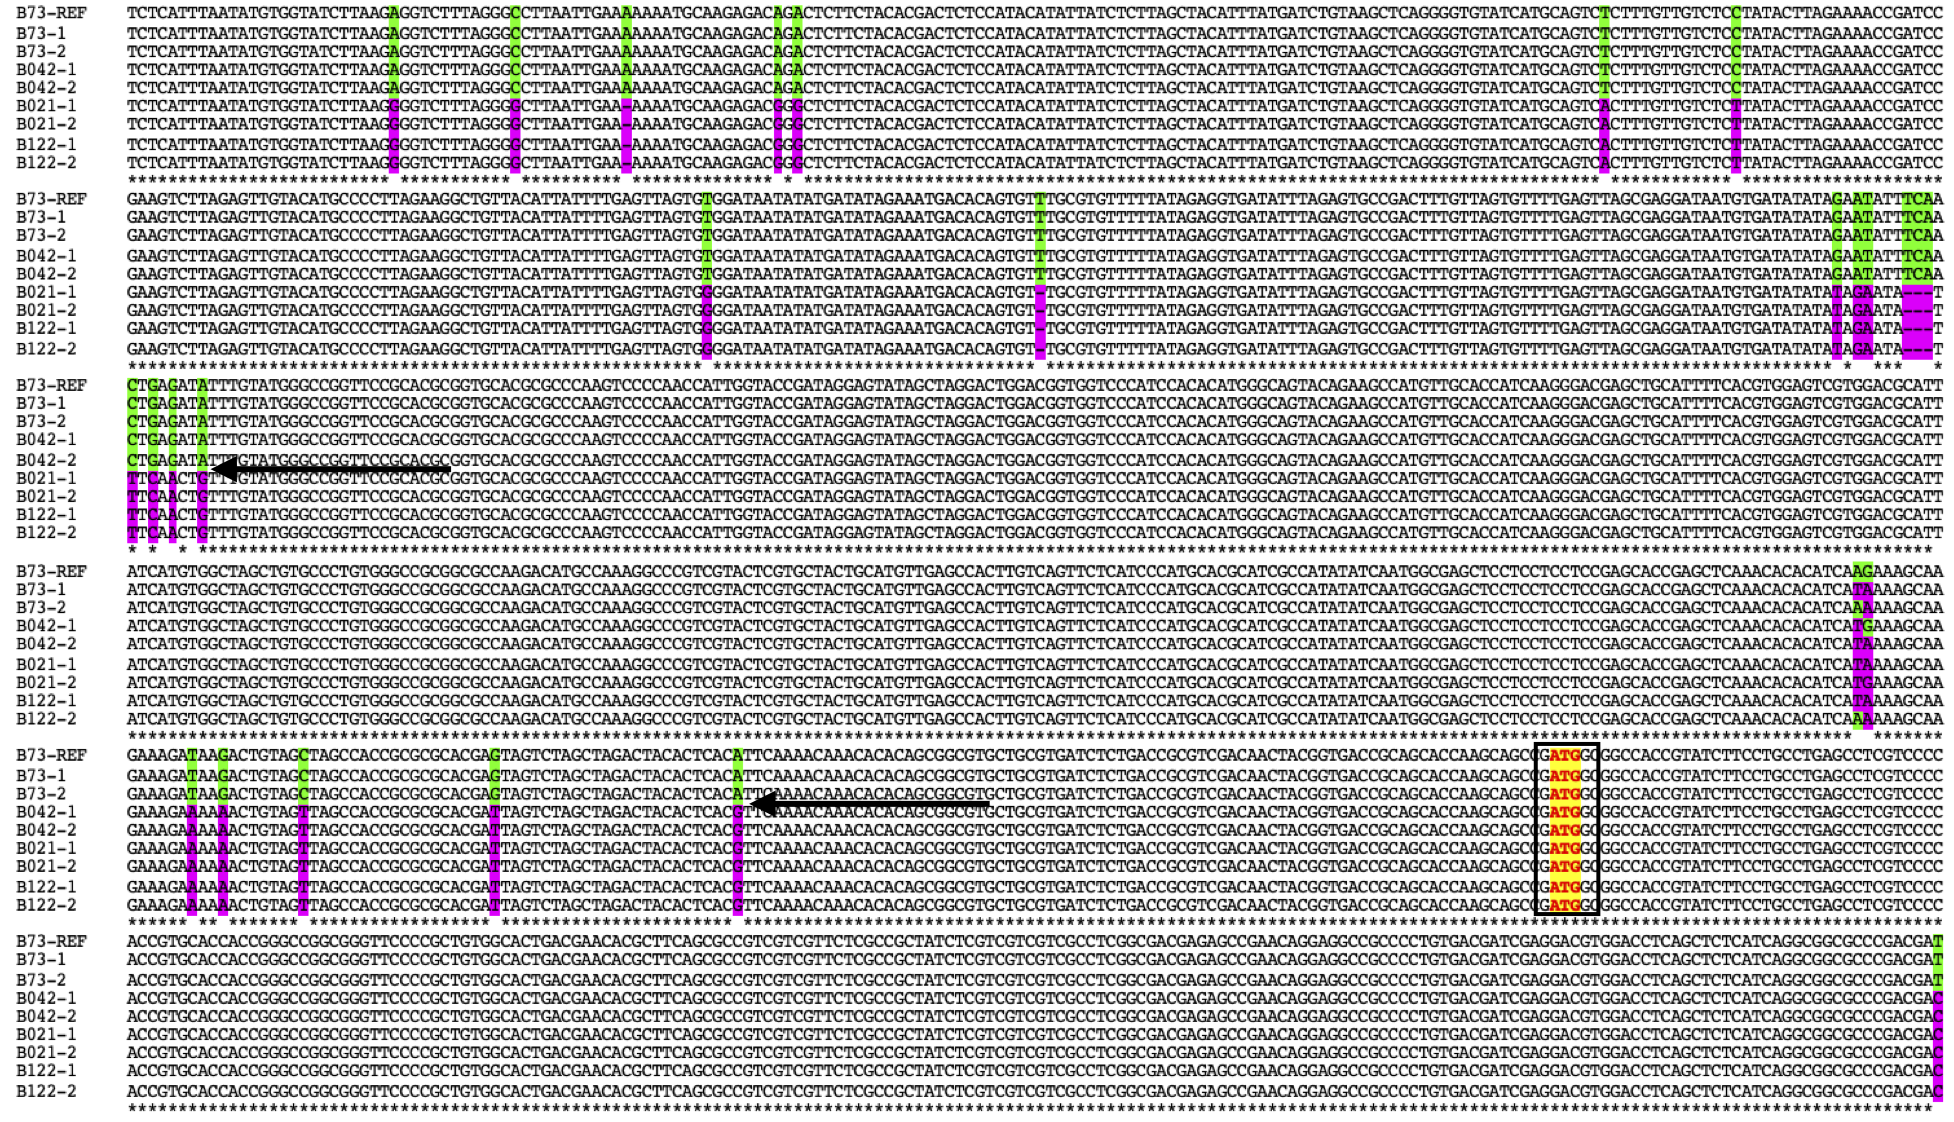
\includegraphics[width=0.8\paperwidth]{Sup_Figures/Sup_Fig_6.png}
\caption{Sanger sequencing of the promoter and start of the \textit{ZmPLA1.2} sequence obtained from B73 plants and 3 BILs (B042, B021 and B122). A recombination point 500 bp upstream the ATG in B104 is indicated by arrows. B73 alleles are marked in green and PT alleles are marked in pink}
\label{SupFig5}
\end{center}
\end{figure*} 

\begin{figure}[t]
\begin{center}
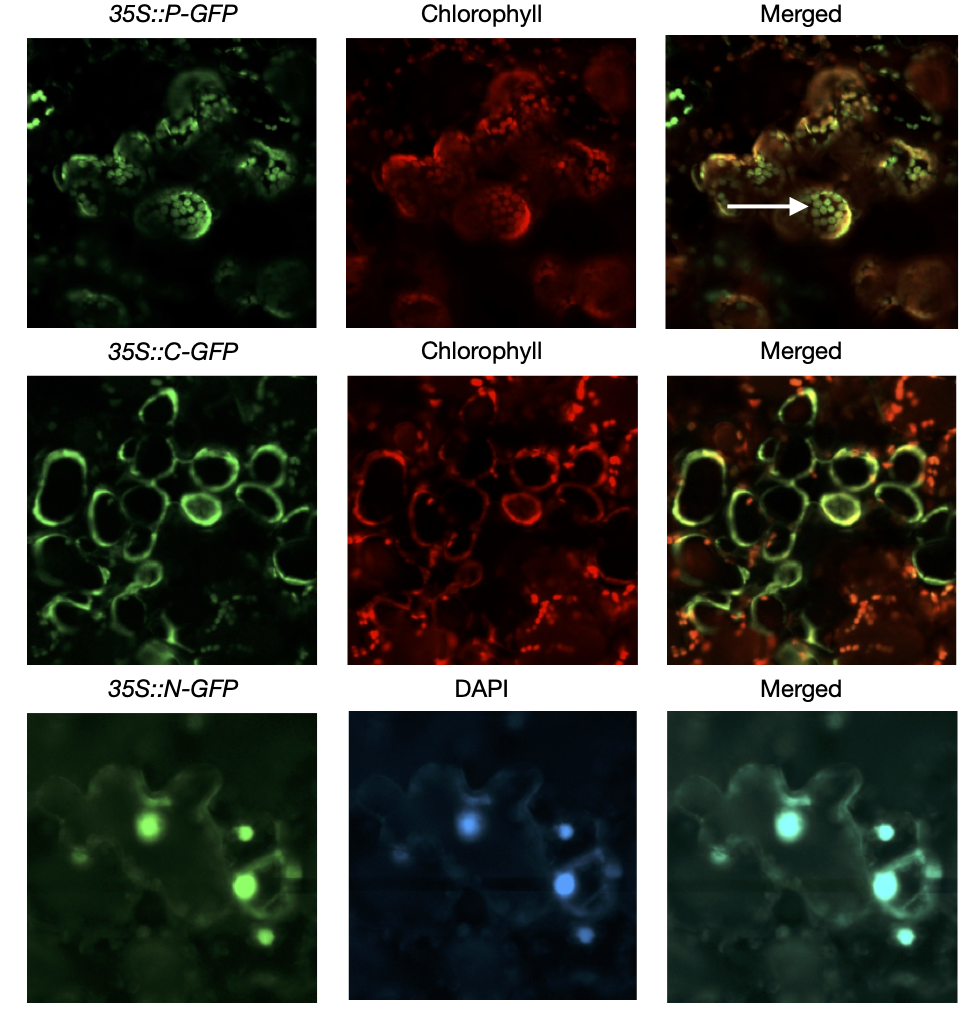
\includegraphics[width=0.8\paperwidth]{Sup_Figures/Sup_Fig_7.png}
\caption{Flowering time and phospholipid related gene expression correlation with flowering time traits in aerial tissues in the 282 panel. 
Data obtained from \cite{Kremling2018-gn}
}
\label{SupFig7}
\end{center}
\end{figure} 

\begin{figure*}[t]
\begin{center}
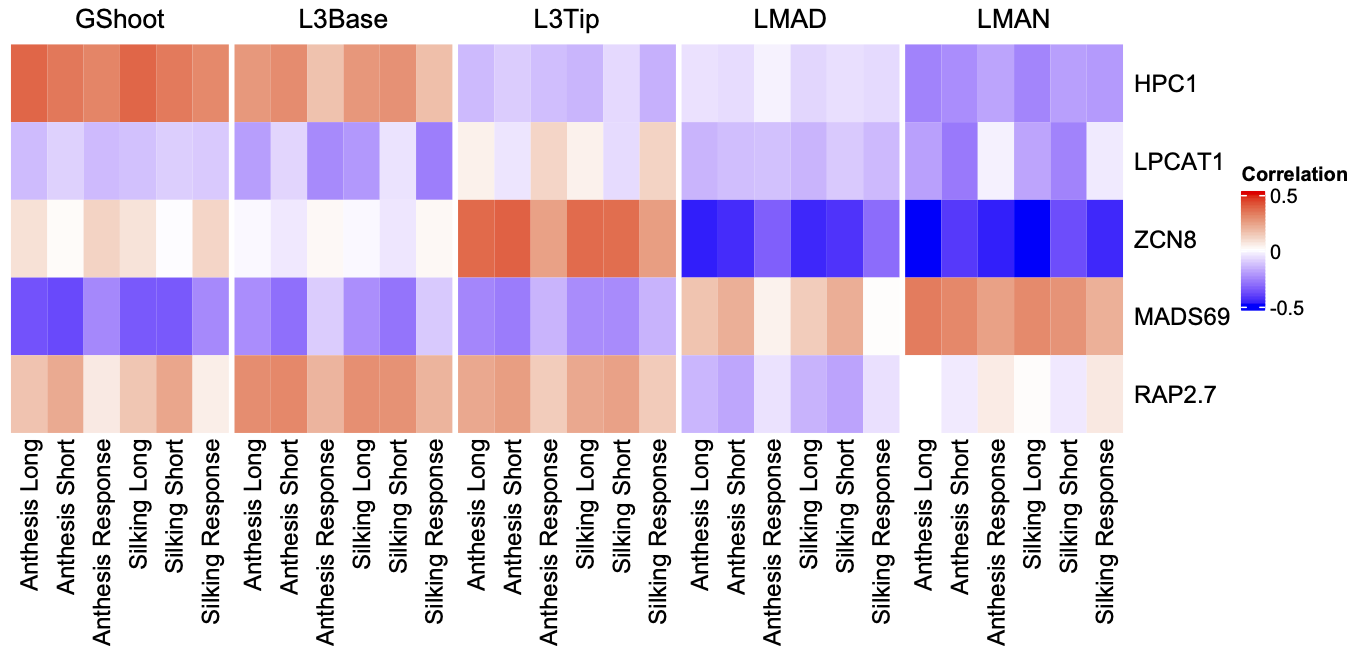
\includegraphics[width=0.8\paperwidth]{Sup_Figures/Sup_Fig_8.png}
\caption{A) Flag leaf hosphorus levels of B73 and 10 highland landraces each from México and Perú grown in control conditions.
B) Andosol soil frequency measured using the geographic coordinates of landrace accessions from the SEEDS dataset calculated using the soilP package \cite{Rodriguez-Zapata2018-vz}.
C) Phosphorus content on the CRISPR \textit{ZmPLA1.2} mutants grown in long day conditions in Raleigh.
D) PCA analysis of ionomics data of the CRISPR \textit{ZmPLA1.2} mutants and control plants grown in long day conditions in Raleigh
}
\label{SupFig8}
\end{center}
\end{figure*} 

\end{document}
